% ======================================== Début Préambule Latex ========================================
% Copyright (c) 2022 Mathis Gauthey
% This source code is licensed under the MIT License found in the
% LICENSE file in the root directory of this source tree.

% ========== Classe du document ==========
\documentclass[a4paper,12pt]{report}    % A4, police taille 11, report pour avoir les chapitres, fleqn pour avoir les équations alignées à gauche

% ========== Langue française pour le document ==========
\usepackage{latexsym}       % Police latex de base

\usepackage[french]{babel}  % Dictionnaire français (indentation, caractères spéciaux, tirets...)
\usepackage[utf8]{inputenc} % Encodage d'entrée pour les caractères accentués
\usepackage[T1]{fontenc}    % Affichage correct des caractères accentués notamment

% ========== Géométrie du document ==========
% Gestion des différentes marges du document pour coller avec le séparateur d'en-tête
\usepackage[left=2cm , right=2cm, bottom=2cm, top=2cm, headheight=2cm, headsep=0.5cm,heightrounded=true]{geometry}
% \raggedbottom % This makes the last line of each page be at exactly the same place on the sheet of paper
% \flushbottom  % All pages will not necessarily have exactly the same height, but ‘almost the same height’
\setlength{\parskip}{1em}   % Définition de l'espace entre les paragraphes
\setlength{\parindent}{2em} % Définition de la longueur du "tab" = indentation
\usepackage{setspace}
\setstretch{1}
\usepackage{fancyhdr}       % Permet en-tête et pied de page
\pagestyle{fancyplain}      % Pour avoir le même style sur les pages fancy et sur celles plains comme la toc
\renewcommand\plainheadrulewidth{.4pt}  % Le trait noir sous les logos sur les pages plain
\fancyhead[L]{
\includegraphics[scale=0.05]{logo_iresne.png}}    % Logo gauche
\fancyhead[R]{
\includegraphics[scale=0.05]{polytech.jpg}} % Logo droit
% Redéfinir le style "empty" utilisé par le documentclass "report" pour le titre, résumé et chapitres
\fancypagestyle{empty}
{
    \fancyhf{}
    \fancyhead[L]{
\includegraphics[scale=0.05]{logo_iresne.png}}    % Logo gauche
    \fancyhead[R]{
\includegraphics[scale=0.05]{polytech.jpg}} % Logo droit
}

% ========== Liens dans le document, méta-datas et références ==========
\usepackage{xpatch}     % Permet de patcher certaines fonctionnalités de base comme la toc
\usepackage{float}      % Placement des flottants
\usepackage{hyperref}   % Liens dans le documents
\usepackage{caption}    % Légendes dans les environnements "figure" et "float"
\usepackage[list=true]{subcaption} % Légendes pour les "sous-figures" et "sous-float"
                                   % et affichage des "sous-..." dans la liste des figures
%\def\thechapter{\Alph{chapter}}    % Définition des chapitres avec une lettre
\setcounter{tocdepth}{3}           % Profondeur de numérotation de la toc  (chap > sec > subsec > subsubsec)
\setcounter{secnumdepth}{3}        % Profondeur de numérotation des titres (chap > sec > subsec > subsubsec)
\usepackage{chngcntr}              % Permet de changer les numérotations d'objets
\usepackage[titles]{tocloft}       % Gestion très précise des différentes listes

\hypersetup % Attribution des méta-datas pdf pour reconnaissance automatique Zotero entre autres
{
pdftitle={Validation d'un code CFD couplant hydrodynamique et transfert de masse},
pdfsubject={Stage5APolytech},
pdfauthor={Clément PLUMECOCQ},
	pdfkeywords={keyword1} {keyword2} {keyword3}
}

% ========== Graphique, police, maths ==========
\usepackage[table,xcdraw]{xcolor}       % Package permettant d'utiliser de la couleur
% \usepackage{color}                      % Rajouter de la couleur au texte
\usepackage{bm}                         % Mettre en gras des maths avec la commande \bm
\usepackage{ragged2e}                   % Meilleure gestion de l'alignement des textes entre autres
\usepackage{tcolorbox}                  % Boite colorées pour texte, images ou équations
\usepackage{textcomp}                   % Symboles et polices
\usepackage{gensymb}                    % Symbole pour le degré entre autre
\usepackage{amsmath,amsfonts,amssymb}   % Écrire des maths
\usepackage{cancel}                     % Barrer des maths
\usepackage{mathtools}                  % Gestion des matrices et de maths complexes
\usepackage{morewrites}                 % Résoud un problème entre les listes équation et codes


\usepackage{lmodern}
\usepackage[Lenny]{fncychap}

\ChNameUpperCase
\ChNumVar{\fontsize{40}{42}\usefont{OT1}{ptm}{m}{n}\selectfont}
\ChTitleVar{\Huge \bfseries}

\usepackage{pifont}
\usepackage{enumitem}       % Gestion des énumérations

% Gestion des espaces avant et après les listes plus agréable à la vue
% \setlist[itemize]{noitemsep, topsep=5pt, before={\vspace*{-\baselineskip}}}
% Si désactivé (commenté), penser à ajouter un \smallskip, \medskip ou \bigskip après un itemize.

\definecolor{bulletcolor}{RGB}{128,128,128}


\usepackage{siunitx}                                    % Pour des unités bien écrites
\newcommand{\nomunit}[1]{%
\renewcommand{\nomentryend}{\hspace*{\fill}#1}}         % Commande pour la nomenclature (unités à droite)
\sisetup{inter-unit-product =\ensuremath{{}\cdot{}}}    % Séparation par un point des unités
\DeclareSIUnit\bar{bar}                                 % Besoin de déclarer les bar car pas pris en charge

\usepackage{contour}
\usepackage[normalem]{ulem}

\renewcommand{\ULdepth}{1.8pt}
\contourlength{0.8pt}

\newcommand{\myuline}[1]{%
	\uline{\phantom{#1}}%
	\llap{\contour{white}{#1}}%
}



% ========== Glossaire ==========
%\usepackage[acronym,toc]{glossaries}    % Gestion d'un glossaire et d'une liste d'acronymes,
%                                        % et ajout dans la toc de la position de ces derniers
%% Pas besoin de points à la fin du document

\newglossaryentry{mot_complexe}{
    name={mot complexe},
    description={Un mot complexe nécessite généralement une explication}}

\newacronym{lfala}{LFALA}{Les Français Aiment Les Acronymes}                        % Récupère les informations du fichier glossary.tex
%\makeglossaries                         % Génère le glossaire avec les informations récupérées

% ========== Nomenclature ==========
\usepackage[intoc]{nomencl}         % Gestion d'une nomenclature avec position dans la toc
\makenomenclature                   % Génère la nomenclature
\usepackage{etoolbox}               % Permet de créer des groupes de nomenclature

% Création de groupes de nomenclature : ATTENTION -> Uniquement des caractères uniques en identifiant
\renewcommand\nomgroup[1]{%
  \item[\bfseries
  \ifstrequal{#1}{A}{Groupe 1}{%
  \ifstrequal{#1}{B}{Groupe 2}{%
  \ifstrequal{#1}{C}{Groupe 3}{%
  }}}%
]} % Attention aux accolades lors de la création de groupes

\AtBeginDocument{   % Nomenclature à générer
\nomenclature[A]{$c_{air}$}{Célérité du son dans l'air à \SI{15}{\celsius} \nomunit{\SI{340.29}{\meter\per\second}}}
\nomenclature[B]{$T_N$}{Période propre de l'élément considéré}
\nomenclature[B]{\(E\)}{{Module d'Young}}
\nomenclature[C]{$\dot{\epsilon}$}{Vitesse de déformation \nomunit{\si{\per\second}}}
}

% ========== Gestion des figures ==========
\usepackage{graphicx}               % Plus d'arguments pour la fonction \includegraphics
\graphicspath{{Images/}}            % Path des images

%\counterwithin{figure}{section}     % Numérotation des figures à partir des sections
\setcounter{lofdepth}{2}            % Afficher jusqu'aux sous-figures dans la liste des figures
\cftsetindents{figure}{0em}{3.5em}  % Réglage de l'espace entre le numéro et le nom de la figure dans la liste
\setlength\cftbeforefigskip{5pt}    % Réglage de l'espacement entre les figures dans la liste
\AtBeginDocument{\renewcommand{\listfigurename}{Liste des figures}} % Renommer la liste des figures
% Ajout de la position de la liste des figures dans la toc
\xpretocmd{\listoffigures}{\addcontentsline{toc}{chapter}{\listfigurename}}{}{}
\usepackage{tikz}
% ========== Gestion des tableaux ==========
\usepackage{array,multirow,makecell}                        % Packages utiles pour les tableaux
\setcellgapes{1pt}                                          % Paramètres sympa d'après Xm1Math
\makegapedcells                                             % Paramètres sympa d'après Xm1Math
\newcolumntype{R}[1]{>{\raggedleft\arraybackslash }b{#1}}   % Paramètres sympa d'après Xm1Math
\newcolumntype{L}[1]{>{\raggedright\arraybackslash }b{#1}}  % Paramètres sympa d'après Xm1Math
\newcolumntype{C}[1]{>{\centering\arraybackslash }b{#1}}    % Paramètres sympa d'après Xm1Math

%\counterwithin{table}{section}      % Numérotation des tableaux à partir des sections
\setcounter{lotdepth}{2}            % Afficher jusqu'aux sous-tableaux dans la liste des tableaux
\cftsetindents{table}{0em}{3.5em}   % Réglage de l'espace entre le numéro et le nom du tableau dans la liste
\setlength\cftbeforetabskip{2pt}    % Réglage de l'espacement entre les figures dans la liste
% Ajout de la position de la liste des tableaux dans la toc
\xpretocmd{\listoftables}{\addcontentsline{toc}{chapter}{\listtablename}}{}{}

% ========== Gestion des équations ==========
\newcommand{\listequationsname}{Liste des équations}    % Renommer la liste des équations
\newlistof{myequations}{equ}{\listequationsname}
\newcommand{\myequations}[1]{%
   \addcontentsline{equ}{myequations}{\protect\numberline{\theequation}#1}
}
\counterwithin{equation}{chapter}           % Numérotation des équations à partir des sections
\cftsetindents{myequations}{0em}{3.5em}     % Réglage de l'espace entre le numéro et le nom de l'équation dans la liste

% Création de la commande \noteworhty pour les équations importantes qui méritent d'être listées
\newcommand{\noteworthy}[2]{
\begin{align} \label{#2} \ensuremath{\boxed{#1}} \end{align}
\myequations{#2}
\begingroup
\centering \small \textit{#2}

\endgroup}

\makeatletter   % Espacement des équations plus important entre les chapitres
\xpretocmd{\@chapter}{\addtocontents{equ}{\protect\addvspace{10\p@}}}{}{}{}%
\makeatother





% ========== Index ==========
\usepackage{imakeidx}   % Package pour créer l'index
\makeindex              % Génération de l'index
% Ajout de la position de l'index dans la toc
\xpretocmd{\printindex}{\addcontentsline{toc}{chapter}{\indexname}}{}{}

% ========== Bibliographie ==========
% Importer un fichier biblatex, sans dépassement des marges, trié par ordre d'apparition
\usepackage[
backend=biber,
style=numeric,
sorting=none
]{biblatex}
\usepackage{csquotes}           % Gestion des caractères " " lors des citations
\addbibresource{biblio.bib}    % Importer le fichier de bibliographie
%\nocite{*}                      % Importer les éléments non cités quand même dans la bibliographie

% ========== Gestion des annexes ==========
\usepackage[toc,page,title,titletoc,header]{appendix}   % Packages indexes importants
\usepackage{pdfpages}                                   % Intégration de pdf dans le document
\renewcommand{\appendixtocname}{Table des annexes}      % Nom de la table des annexes dans la toc
\renewcommand{\appendixpagename}{Annexes}               % Nom du titre de la page des annexes
\usepackage{titletoc}	% Permet de générer une petite table des annexes

% ========== Utilitaires ==========
\usepackage[all,defaultlines=3]{nowidow}    % Macro pour la gestion des lignes seules en bout de page
\usepackage{blindtext}                      % Génération de texte aléatoire pour les exemples
% A utiliser avec https://ctan.mirror.garr.it/mirrors/ctan/macros/latex/contrib/mwe/mwe.pdf pour les images

% Paquets et commande perso clement plumecocq
\usepackage{bm}
\newcommand{\M}{\mathbb}					
\newcommand{\Mb}{\mathbf}									
\newcommand{\Mc}{\mathcal}
\newcommand{\grad}[1]{\nabla #1}
\renewcommand{\div}[1]{\nabla \cdot \left(#1\right)}
\newcommand{\Lapl}[1]{\Delta #1}
\newcommand{\boundary}[1]{\partial \domain{#1}}
\newcommand{\doubleoverline}[1]{\bar{\bar{#1}}} 			% notation matrice
\newcommand{\co}[1]{\text{cos}\left(#1\right)}
\newcommand{\sinus}[1]{\text{sin}\left(#1\right)}




% ======================================== Fin Préambule Latex ========================================

% ======================================== Début TUTOs ========================================

% ========== Intégrer une image ==========
%\begin{figure}[htbp]
%\centering
%\includegraphics[width=\textwidth]{example-image-a.png}
%\caption{Image A}
%\label{fig:example-image-a} % Bon réflexe de garder le même nom de fichier et de label
%\end{figure}

% ========== Insérer de multiples images ==========
% \begin{figure}[H]
%     \begin{subfigure}[t]{0.475\textwidth}
%         \includegraphics[width=1\textwidth]{example-image-b}
%         \caption{Image B}
%         \label{subfig:example-image-b}
%     \end{subfigure}%
%     ATTENTION, le % est très important ici pour éviter les problèmes de vide
%     \hfill    % Remplissage entre les images
%     \begin{subfigure}[t]{0.475\textwidth}
%         \includegraphics[width=1\textwidth]{example_image_c}
%         \caption{Image C}
%         \label{subfig:example-image-c}
%     \end{subfigure}
%     \caption{Exemple d'utilisation des sous-figures}
%     \label{fig:test_subfigure}
% \end{figure}

% ========== Placement des images ==========
% h Place the float here, i.e., approximately at the same point it occurs in the source text (however, not exactly at the spot)
% t Position at the top of the page.
% b Position at the bottom of the page.
% p Put on a special page for floats only.
% ! Override internal parameters LATEX uses for determining "good" float positions.
% H Places the float at precisely the location in the LATEX code. Requires the float package (\usepackage{float}). This is somewhat equivalent to h!, though some errors may arise if you have too many consecutive floats with [H].

% ========== Intégrer un tableau ==========
% https://www.tablesgenerator.com/

% ========== Intégrer une équation ==========
% https://editor.codecogs.com/
% \noteworthy{equation}{légende} pour l'avoir dans la liste des équations

% ========== Intégrer du code ==========
% \begin{listing}[htbp]
% \begin{minted}{c}
% #include <stdio.h>
% int main() {
%   printf("Hello, World!"); /*printf() outputs the quoted string*/
%   return 0;
% }
% \end{minted}
% \caption{Hello World in C}
% \label{listing:2}
% \end{listing}

% \mint{python}|print("hello")| % Équivalent de \minted mais plus court

% \mintinline{python}|print("hello")|   % Quand t'as qu'une ligne de code

% Remarque : Le séparateur aurait pu être { } ou d'autres ponctuations

% \inputminted[firstline=2, lastline=12]{octave}{BitXorMatrix.m}

% ========== Début de doc classique ==========
% \title{Titre}
% \author{Auteur}
% \date{\today}
% \maketitle
% \begin{abstract}
%     Blablabla
% \end{abstract}

% ======================================== Fin TUTOs ========================================
%---AUTRES PAQUETS---
%%%%% OPTIONS TIKZ
\usetikzlibrary{arrows.meta}
\usetikzlibrary{shapes}
\begin{document}

% ======================================== Début Page de Garde ========================================

\hypersetup{pageanchor=false}
\begin{titlepage}
    \begin{center}
        \vspace*{1cm}

        \Huge
        \textbf{Validation d'un code CFD couplant hydrodynamique et transfert de masse}

        \vspace{0.5cm}
        \LARGE
        Commisariat à l'énergie atomique et aux énergies alternatives \\
        Laboratoire de Modélisation des Accidents Graves, LMAG\\
        \Large Cadarache 13115 Saint-Paul-lèz-Durance\\
         27/02/2023 - 11/08/2023
        \vspace{1.5cm}

        \textbf{\LARGE Clément Plumecocq}

        \vfill

        
\includegraphics[scale=0.15]{logo_iresne.png}
\includegraphics[scale=0.20]{polytech.jpg}
        \vfill
        \Large
        \noindent%\fbox{\begin{minipage}[c][0.3\textwidth]{\textwidth-7pt}%
        %\begin{center}
        POLYTECH Marseille - Mécanique Énergétique \\ \vfill
        %\par\end{center}
        %\begin{center}
        Maître de stage : Romain Le Tellier, Ingénieur-Chercheur LMAG \\
        Encadrant : Mirantsoa-Aimé Rasolofomanana, Doctorant LMAG \\
        Tuteur école : Marc Médale, Professeur des universités IUSTI-AMU
        %\par\end{center}
        %\end{minipage}}
    \end{center}
\end{titlepage}

% ======================================== Fin Page de Garde ========================================

% ======================================== Début Page Résumé ========================================

% French

\thispagestyle{empty}
\begin{center}
    \Large


    \vspace{0.9cm}
    \textbf{Résumé}
\end{center}

\blindtext

\begin{center}
	\Large
	\vspace{0.9cm}
	\textbf{Abstract}
\end{center}

\blindtext

% ======================================== Fin Page Résumé ========================================

% ======================================== Début TOC & Co ========================================

\newpage
%\hypersetup{pageanchor=true}
\renewcommand{\baselinestretch}{0.}\normalsize
\tableofcontents
\renewcommand{\baselinestretch}{1.0}\normalsize






\newpage
\printnomenclature

% ======================================== Fin TOC & Co ========================================

% ======================================== Début Document ========================================

\newpage

\section*{Remerciements}
\setcounter{page}{1}
\chapter{Éléments théoriques sur la méthode de champ de phase} \label{chap:2}
Ce deuxième chapitre résume l'ensemble des notions théoriques liées à la méthode champ de phase. Le couplage avec l'hydrodynamique est présenté puis une description analytique de l'énergie ainsi que les principales hypothèses du modèle sont introduites. 
\section{Présentation des principales méthodes de suivi et de capture d'interface}

Le traitement numérique efficace des interfaces représente un enjeu majeur de la simulation numérique tant les applications faisant intervenir des interfaces sont importantes. On différencie les méthodes de suivi d'interface des méthodes de capture d'interface. Les méthodes de suivi d'interface suivent des marqueurs placés sur l'interface au cours du temps, la position de l'interface est alors explicite. Les méthodes de capture d'interface quant à elle suivent implicitement l'interface au travers de l'évolution d'une fonction couleur. De nombreuses méthodes existent, on présente ici les principales :
\begin{itemize}
	\item[$\bullet$] \textit{\textbf{Volume of fluid (VOF) : }} Cette méthode utilise un maillage fixe découpé en cellule représentant des volumes. On associe alors à chacune de ces cellules une fraction volumique de fluide, cette proportion est alors résolue au cours du temps et la position de l'interface peut être reconstruite. Cette reconstruction a pour désavantage de ne fournir que peu d'informations viables sur l'interface. Cette méthode reste donc peu précise et est également difficile à mettre en \oe uvre en trois dimensions.
	\item[$\bullet$] \textit{\textbf{Méthode Level-Set (LS) : }}	Cette méthode repose sur la résolution implicite de l'interface au travers de la résolution d'une fonction auxiliaire dite fonction ligne de niveau, généralement la distance signée à l'interface. Cette fonction se doit d'admettre une valeur nulle à l'interface, ainsi au travers de la résolution d'une équation d'advection sur cette fonction ligne de niveau, l'interface est résolue. Cette méthode convient pour les problèmes à fort changement topologique mais présente le désavantage d'être non-conservative.
	\item[$\bullet$]\textit{\textbf{Arbitrary Lagrangian-Eulerian (ALE) : }} La méthode repose sur une double description lagrangienne (maillage mobile) et eulérienne (maillage fixe), à chaque itération temporelle, le maillage autour de l'interface est reconstruit pour s'adapter à la forme de l'interface, ainsi chaque maille contient uniquement un fluide. L'ensemble de ces propriétés rend la méthode très précise mais difficile à mettre en \oe uvre en trois dimensions.
	\item[$\bullet$]\textit{\textbf{Front-Tracking (FT) : }} La méthode utilise des marqueurs sans masse positionnés sur l'interface transportée suivant une description lagrangienne sur un maillage eulérien fixe. Ainsi les équations de Navier-Stokes sont résolues sur un maillage fixe tandis que l'équation régissant la position de l'interface est résolue sur un maillage mobile. La principale difficulté réside dans le choix des opérateur de communication entre les deux maillages. Cette méthode nécessite l'implémentation d'algorithme pour les cas de coalescence et rupture d'interface et possède comme désavantage de ne pas être conservative.
\end{itemize}








\section{Méthode champ de phase conservative}
\subsection{Présentation générale}
%Les méthodes de suivi ou de capture d'interface présentées précédemment décrivent toute l'interface comme une discontinuité, cependant il existe un second paradigme traitant l'interface comme une zone de transition continue, on parle alors d'interface diffuse. \\
Le traitement numérique de l'interface présente deux paradigmes : le premier traite l'interface comme une discontinuité. Le second modélise l'interface comme une zone de transition continue, on parle alors d'interface diffuse.
Dans ce second cas l'interface correspond donc à une zone d'épaisseur connue et maîtrisée où cohabitent les deux phases, les gradients à l'interface étant finis le traitement numérique est alors facilité. Ce concept d'interface diffuse date du XIX$^{\text{ème}}$siècle et est introduit par Van Der Walls \cite{rowlinson_translation_1979}.
\begin{figure}[H]
	\centering
	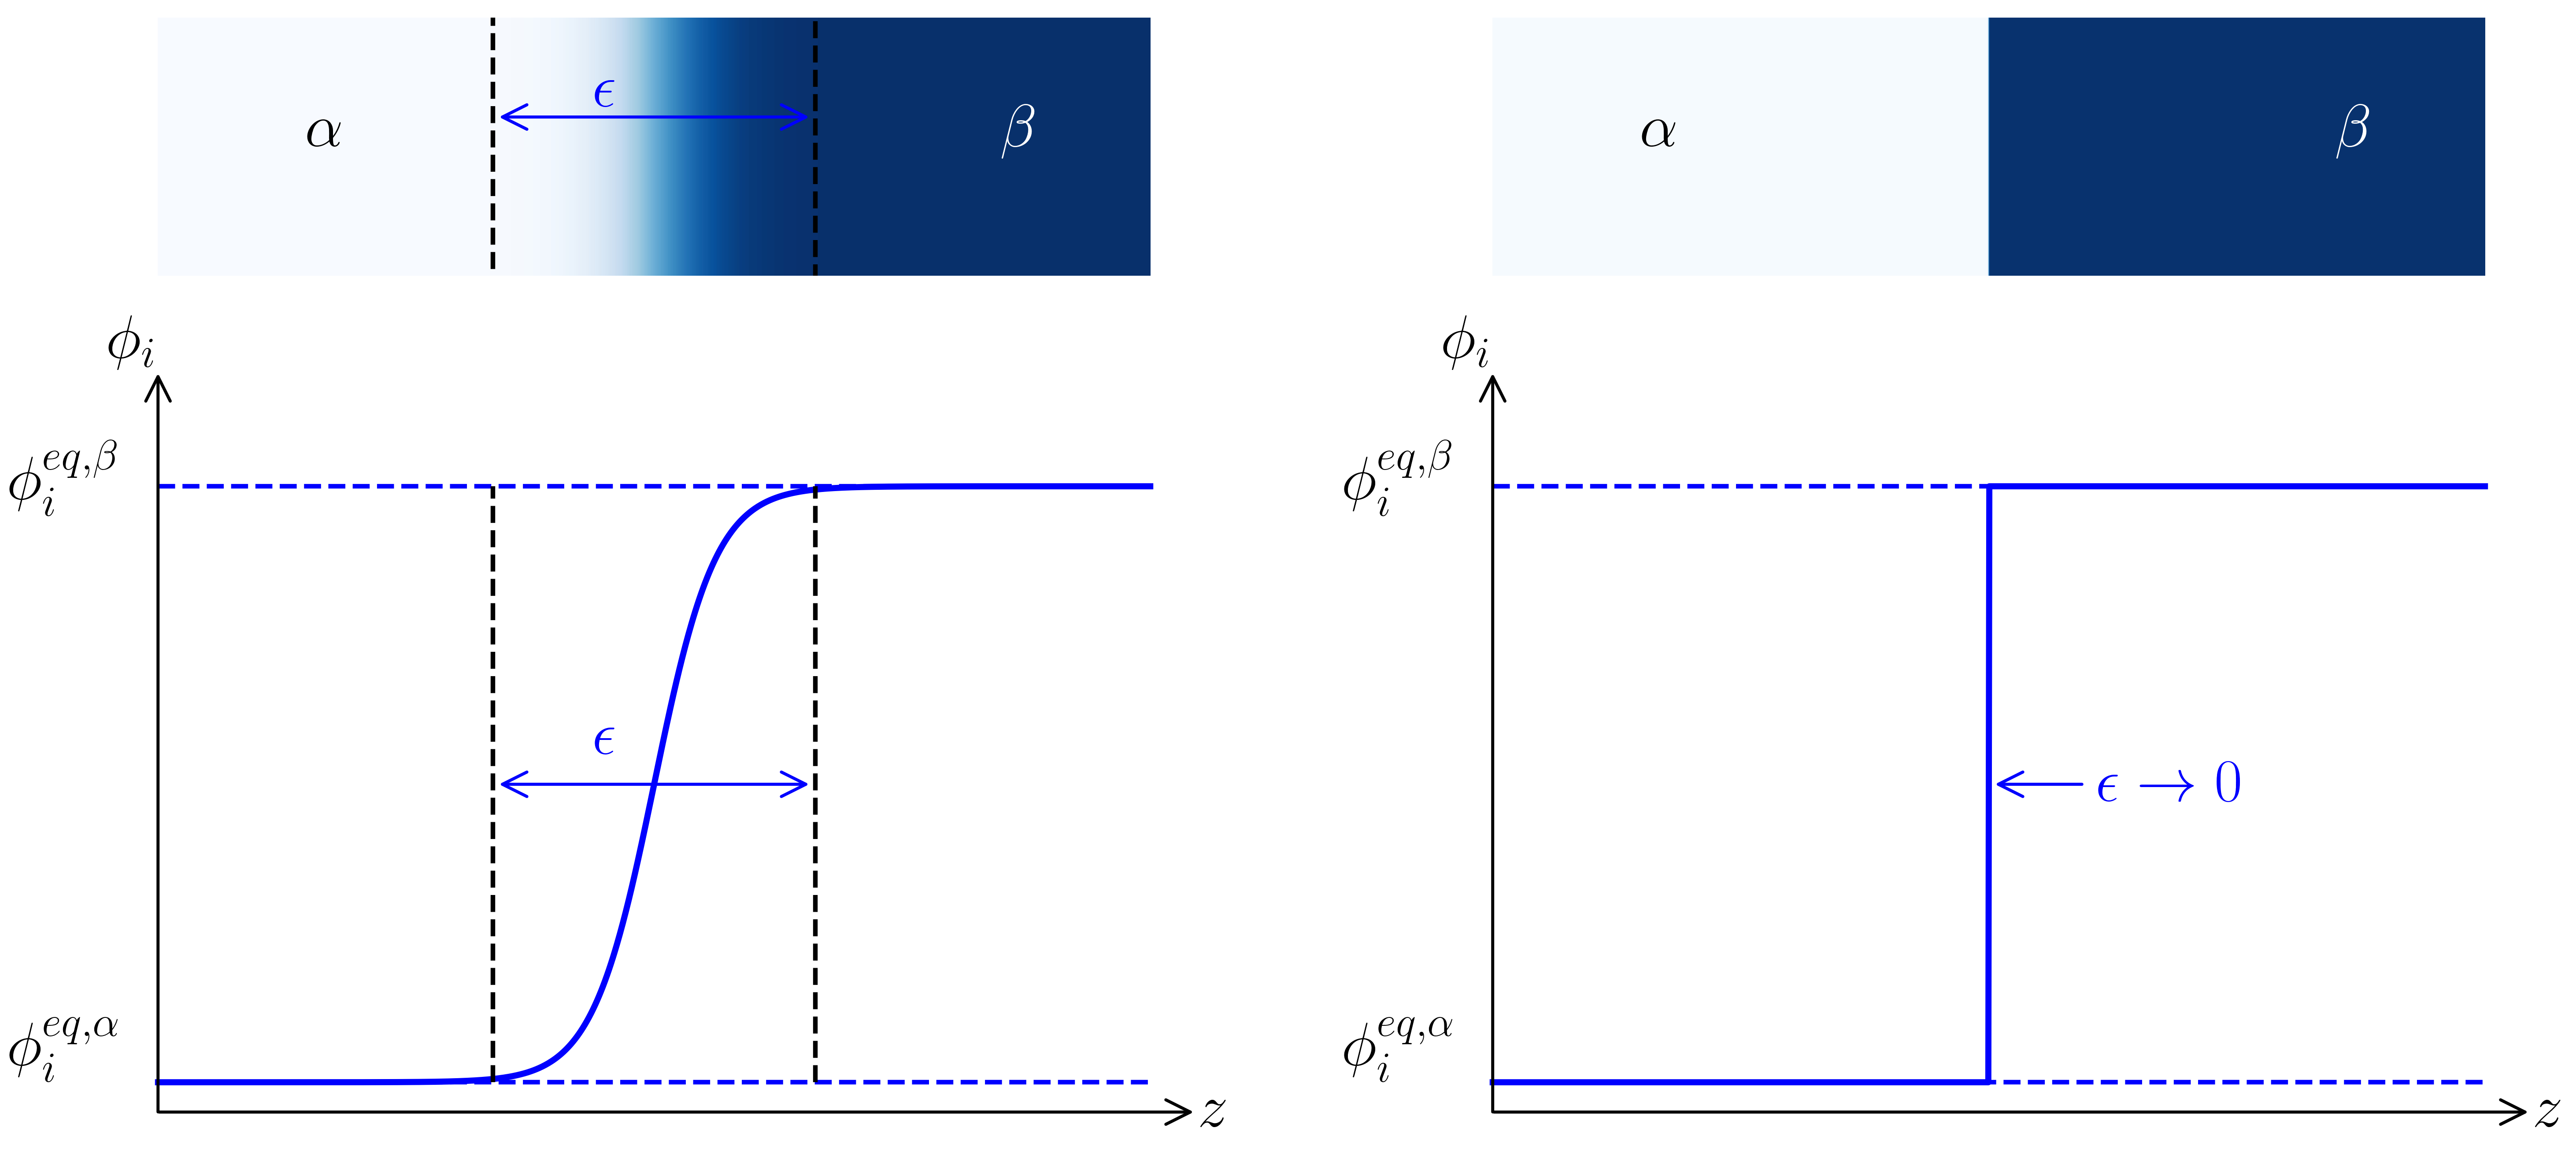
\includegraphics[width=0.5\linewidth]{figure/diffuse_interface}
	\caption{Comparaison entre une interface diffuse (à gauche) et une interface raide (à droite)}
	\label{fig:diffuseinterface}
\end{figure} 
 Le concept d'interface diffuse va gagner l'intérêt de la communauté scientifique avec le développement de la méthode champ de phase. En 1950, Ginzburg et Landau propose une description de l'énergie libre d'un système tenant compte des inhomogénéités spatiales (interfaces) en fonction d'un paramètre d'ordre \cite{landau_physique_1995}. En 1958, Cahn et Hilliard \cite{cahn_free_1958}  introduisent l'utilisation de cette description pour décrire l'évolution de la composition. Ces études sont la base de la méthode champ de phase. En effet la méthode champ de phase est basée sur la représentation d'un système au travers d'une fonctionnelle d'énergie libre, la description diffuse de l'interface et le suivi de paramètres d'ordre $\phi$. La méthode champ de phase est aujourd'hui utilisée dans de nombreux domaines, certains sont présentés en figure \ref{fig:champphase}.
\begin{figure}[H]
	\centering
	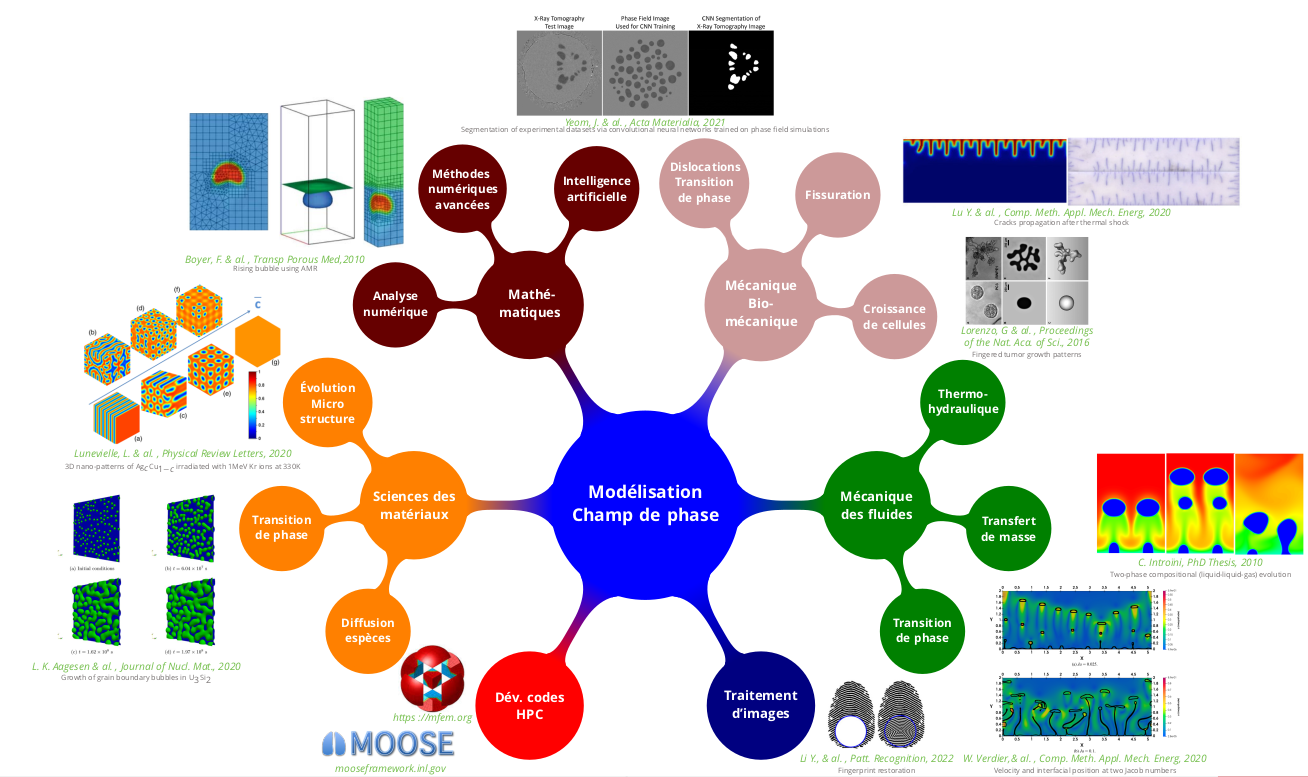
\includegraphics[width=0.9\linewidth]{figure/champ_phase}
	\caption[Domaine d'application de la méthode champ de phase]{Domaine d'application de la méthode champ de phase, tirée de \cite{introini_suivi_nodate}}
	\label{fig:champphase}
\end{figure} 
\subsection{Équation de Cahn-Hilliard généralisée}
Dans le cas n-composants on note $\{\phi_i\}_{i=1,..n}$ \footnote{Par soucis de simplification on pourra également utiliser la notation $\{\phi\}$} l'ensemble des paramètres d'ordre du système. Ces paramètres peuvent représenter la concentration, la fraction massique ou d'autres grandeurs.
Comme expliqué précédemment la méthode de champ de phase repose sur le suivi de ces variables. Ces paramètres d'ordre peut être conservés ou non, dans notre étude les paramètres d'ordres sont conservés. De plus on considère un système fermé, ainsi on obtient la contrainte :
\begin{equation}
\sum_{i=1}^n \phi_i =1 \Rightarrow \phi_n =1 - \sum_{i=1}^{n-1} \phi_i
\end{equation} 
Ainsi pour un mélange à $n$ composants, cette loi de fermeture permet de décrire l'ensemble du système en suivant l'évolution d'uniquement $n-1$ composants. Dans certains cas le système peut également être décrit avec des variables non conservées telles que des indicatrices de phases ou des grandeurs liées à des réactions chimiques. Le comportement de ces variables est alors régis par des équations de réaction-diffusion dites d'Allen-Cahn, non résolue dans cette étude. Dans le cadre de variables conservées les équations de Cahn-Hillard pour $n$ composants, avec $i\in \{1,..,n-1 \}$ s'écrivent sous la forme :
\begin{equation}
	\cfrac{\partial \phi_i}{\partial t} + \left(\mathbf{u} \cdot \nabla\right) \phi_i =  \nabla \cdot \left(\sum_{j=1}^{n-1}{\mathcal{M}_{ij}} \nabla\left( \frac{\delta \mathbb{F}}{\delta \phi_j}\right) \right) 
\end{equation}
avec : $\mathcal{M}_{ik}$ les coefficient de la mobilité (paramètre cinétique),  $\phi_i$ le paramètre d'ordre, $\mathbf{u}$ la vitesse et $\mathbb{F}$ une fonctionnelle de Ginzburg-Landeau généralisée \cite{cardon_modelisation_2016} définit tel que : 
 \begin{equation}
\mathbb{F}[\{\phi\}] = \int_{\mathcal{V}}\lambda\tilde{g}^{}(\{\phi\},\mathbf{x},t)+ \sum_{i=1}^{n-1}\sum_{j=1}^{n-1}\cfrac{1}{2}\kappa_{ij}\nabla \phi_i \cdot \nabla \phi_j dV
\end{equation}
Avec $\mathbf{x}$ le vecteur position et $V$ le volume.
Le premier terme représente la densité d'énergie liée aux valeurs locales de composition, traduisant l'équilibre des phases ainsi que leurs existences ou coexistence. Pour deux phases $\alpha$ et $\beta$, on rappelle les conditions données par l'équilibre thermodynamique \cite{kim_phase-field_1999} :
\begin{subequations}
	\label{eq:all}
	\begin{empheq}[left={\empheqlbrace\,}]{align}
		&\lambda\left.\frac{\partial \tilde{g}^{}}{\partial \phi_i}\right|_{\phi_i^{\alpha,eq}} = \lambda\left.\frac{\partial \tilde{g}^{}}{\partial \phi_i}\right|_{\phi_i^{\beta,eq}} = \tilde{\mu}_i^{eq} \\
& 		\lambda\tilde{g}^{\alpha,eq} - \sum_{i=1}^{n-1}\tilde{\mu}_i^{eq}\phi_i^{\alpha,eq} = 	\lambda\tilde{g}^{\beta,eq} - \sum_{i=1}^{n-1}\tilde{\mu}_i^{eq}\phi_i^{\beta,eq}
	\end{empheq}
\end{subequations}
$\tilde{\mu}_i^{eq}$ représente un potentiel de diffusion de l'élément $i$ à l'équilibre.\\
Le second terme représente la contribution des interfaces, le coefficient $\kappa_{ij}$, dit coefficient de gradient, tient compte du coût énergétique engendré par l'interface, par la suite ce paramètre pourra être relié à la tension de surface. \\
%Dans le cas binaire il est possible de décrire géométriquement l'ensemble des variables : 
%\begin{figure}[H]
%	\centering
%	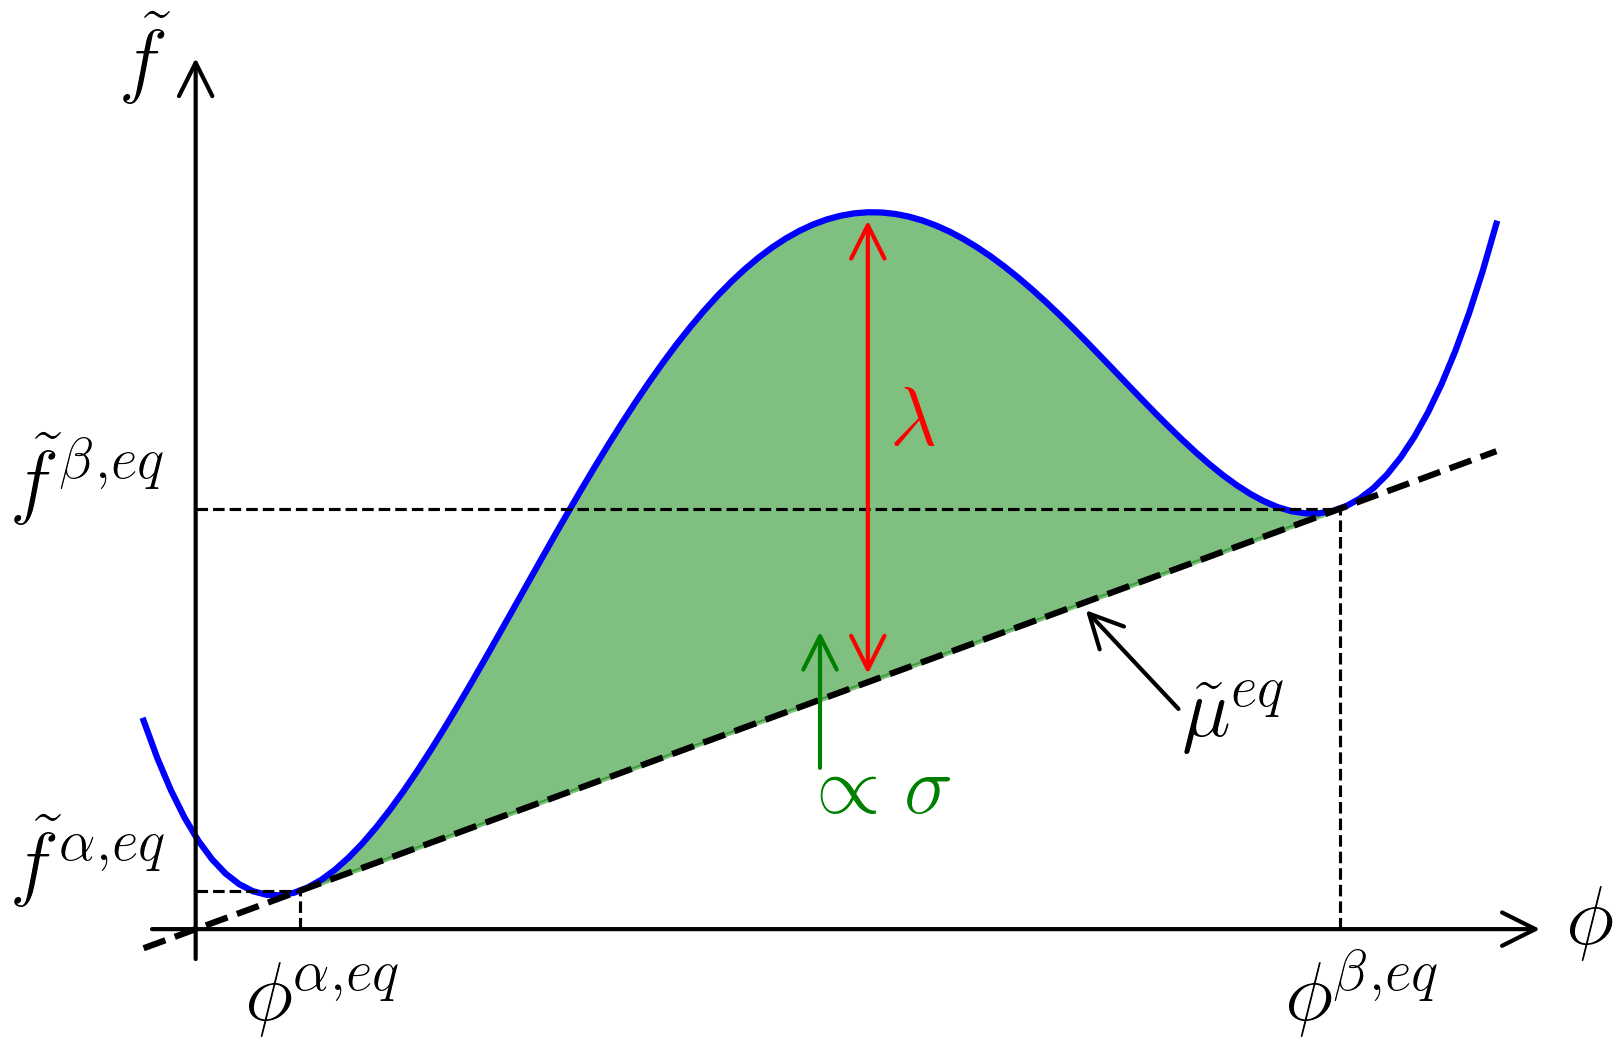
\includegraphics[width=0.45\linewidth]{figure/fig_NRJ}
%	\caption{Description de l'énergie libre pour un système binaire}
%	\label{fig:fignrj}
%\end{figure}
Finalement la dérivée variationnelle de cette fonctionnelle d'énergie libre peut être définie comme un potentiel de diffusion $\tilde{\mu}$: 
\begin{equation}\label{eq_potentiel}
	\frac{\delta \mathbb{F}}{\delta \phi_j} =\lambda \frac{\partial \tilde{g}}{\partial \phi_j} -\sum_{k=1}^{n-1} \kappa_{jk} \Delta \phi_k = \tilde{\mu}_j
\end{equation}
avec $\lambda$ un paramètre d'\textit{upscaling} numérique ajouté pour augmenter l'épaisseur de l'interface. Cet élargissement de l'interface permet d'utiliser des maillages réalistes compte tenu des capacités de calcul actuelles. \\
Le potentiel de diffusion peut être relié au potentiel chimique classique tel que :
%\begin{equation}
%	\tilde{\mu}_i = \frac{\lambda}{V_m}\left(\mu_i - \mu_n\right)
%\end{equation}
\begin{subequations}
	\begin{empheq}[left={\empheqlbrace\,}]{align}
	&\tilde{\mu}_i = \frac{\lambda}{V_m} \hat{\mu}_i \\
		& \hat{\mu}_i = \mu_i - \mu_n
	\end{empheq}
\end{subequations}
Avec $\tilde{\mu}_i$ (en J.m$^{-3}$) représente le potentiel de diffusion volumique de l'élément $i$, $\hat{\mu}_i$ (en J.mol$^{-1}$) le potentiel de diffusion molaire et $V_m$ le volume molaire supposé constant dans tout le système. \footnote{Dans le cadre de ce rapport on note $\tilde{.}$ les grandeurs volumiques}\\
%Le potentiel chimique étant classiquement définit tel que :
%\begin{equation}
%	\mu_i = \left.\frac{\partial G}{\partial n_i}\right|_{P,T,n_{j\neq i }} = \left.\frac{\partial F}{\partial n_i}\right|_{V,T,n_{j\neq i }}
%	  \textrm{                        où           } F = V_m f_0
%\end{equation}
%Avec $F$ (resp. $G$) l'énergie libre d'Helmotz (resp. Gibbs) (en J) et $n_i$ la quantité de matière de l'élément $i$ (en mol). Dans notre cas on se place dans une transformation isobare et isotherme, on privilégiera donc l'énergie de libre de Gibbs.
Dans le cas où $\doubleoverline{\kappa}$ = $\doubleoverline{0}$ on retrouve une équation d'advection-diffusion classique, dans le cas contraire on obtient une équation d'ordre 4. Pour un système binaire le gradient d'energie et le paramètre d'\textit{upscaling} peuvent être déterminés analytiquement. Dans le cas d'une modélisation à n-composants cette approche analytique ne fonctionne plus. Ainsi une des principales difficultés de la mise en place de la méthode champ de phase dans les cas n-aire est l'obtention de ces paramètres.
Dans la suite de ce travail nous utiliserons une proposition de paramétrage introduite par \cite{rasolofomanana_numerical_nodate} et présentée en annexe \ref{ann:parametrage}. Cette paramétrisation permet de déterminer les paramètres d'\textit{upscaling} $\lambda$ et le gradient d'énergie $\bm{\bar{\bar{\kappa}}}$ en fonction des paramètres physiques du système, la tension de surface $\sigma$ et l'épaisseur d'interface $\epsilon$. Ce paramétrage est construit de façon à être consistant vis-a-vis d'un système binaire.
\begin{subequations}
	\label{eq:all}
	\begin{empheq}[left={\empheqlbrace\,}]{align}
	&\bm{\bar{\bar{\kappa}}} = \frac{\sigma \epsilon}{\xi_1 \xi_2}\delta_{ij}
	\label{eq:1} \\
	&\lambda=\frac{\xi_2 \sigma}{2\epsilon\xi_1}
	\label{eq:2}
	\end{empheq}
\end{subequations}
avec $\xi_1 ,\xi_2$ deux constantes dépendantes de la description thermodynamique adoptée, $\delta_{ij}$ le symbole de Kronecker.
\subsection{Couplage avec les équations de Navier-Stokes incompressible}
Dans le cadre de cette étude, les équations de Cahn-Hilliard sont couplées aux équations de conservation de masse et de quantité de mouvement incompressible. Kim J. \cite{kim_phase-field_2012} présente un modèle \textit{one fluid} avec densité variable dans le terme de flottabilité. Les équations de Navier-Stokes s'écrivent sous la forme :
\begin{subequations}
	\label{eq:all}
	\begin{empheq}[left={\empheqlbrace\,}]{align}
	&\nabla \cdot \mathbf{u} = 0\\
	&\rho^* \left (\frac{\partial \mathbf{u}}{\partial t} + (\mathbf{u} \cdot {\nabla})\mathbf{u}\right) = -{\nabla} P +\eta \Delta \mathbf{u}+\sum_{i=1}^{n-1} \tilde{\mu}_i{\nabla} \phi_i + \rho\left(\{\phi_i\}\right) \mathbf{g}
	\end{empheq}
\end{subequations}
avec $\mathbf{u}$ la vitesse, $P$ la pression, $\mathbf{g} = \{ 0,0,-g\}^T $, $\eta$ la viscosité dynamique supposée constante, $\rho^*$ la masse volumique du solvant, $\rho\left(\{\phi_i\}\right)$ une loi de densité fonction du paramètre d'ordre. \\
L'hypothèse du volume molaire constant nous impose que la loi de densité soit une combinaison linéaire des masses volumiques des corps purs que l'on écrit sous la forme : 
\begin{equation}
	\rho\left(\{\phi_i\}\right) = \rho(\phi_n)\left(1+\sum_{i=1}^{n-1}\beta_i \phi_i\right)
\end{equation}
Les paramètres $\beta_i$ sont à déterminer en fonction du système étudié, $\rho(\phi_n)$ correspond à une masse volumique de référence, généralement celle du solvant.
\section{Paysage thermodynamique analytique}
\subsection{Introduction d'un pseudo-grand potentiel}
L'objectif présenté dans \cite{rasolofomanana_numerical_nodate} est d'obtenir une formulation analytique du terme homogène de la fonctionnelle de Ginzburg-Landau. Dans le cas binaire, cette contribution est de la forme d'un double puits, généralement un polynôme de degré 4.
L'objectif est de généraliser ce double puits pour un système n-aire, ainsi on introduit un pseudo grand potentiel correspondant à la hauteur énergétique nécessaire pour changer de minimum d'énergie \cite{cardon_modelisation_2016}.
\begin{equation}
\Omega^{\star} =\Omega - \Omega^{eq} =  {g} - \sum_i \hat{\mu}_i^{eq}\phi_i - \left(  {g}^{eq} -  \sum_i \hat{\mu}_i^{eq}\phi_i^{eq} \right) 
\end{equation}
avec ${g}^{}$ l'énergie libre de Gibbs (J.mol$^{-1}$)\footnote{En utilisant l'hypothèse du volume molaire constant il est possible d'écrire $\tilde{g} = {g}/{V_m}$}, utilisé comme grandeur d'intérêt ici puisque le système est supposé isotherme et isobare.
	\subsection{Application pour un cas diphasique ternaire}
Comme présenté au chapitre \ref{chap:1} le cas d'intérêt de l'étude est le corium. Ce système comprend deux phases à l'équilibre et donc deux points d'équilibre distinct.  Ainsi \cite{rasolofomanana_numerical_nodate} introduit une formulation sous la forme d'un double puits de la forme :
\begin{equation}\label{double_puit}
	\Omega^{\star}  = P^{dis} \times P^{cont}
\end{equation}
Où $P^{dis}, P^{cont}$ représentent deux paraboloïdes correspondant aux deux phases en présence à l'équilibre notées dispersée (ou drop) et continue. Dans le cas ternaire, en considérant les éléments d'intérêt notés miscible ($misc$)  et immiscible ($immi$)  : 
\begin{multline}
P^{k}=\left(\frac{\co{\theta^{k}}(\phi_{misc}-\phi_{misc}^{eq,k}) + \sinus{\theta^{k}}(\phi_{immi}-\phi_{immi}^{eq,k})}{a_{misc}^{k}}\right)^{2}+\\ \left(\frac{-\sinus{\theta^{k}}(\phi_{misc}-\phi_{misc}^{eq,k}) + \co{\theta^{k}}(\phi_{immi}-\phi_{immi}^{eq,k})}{a_{immi}^{k}}\right)^{2}
\label{eq:paraboloid_general_}
\end{multline}
Avec $k = \{disp,cont\}$ la phase (dispersée ou continue), $a_{misc}^k$ (resp. $a_{immi}^k$) le demi-petit (resp. demi-grand) puits, $\theta^k$ l'angle de rotation associé au puits de la phase $k$.\\
On trace alors en exemple le cas le plus simple de paysage :
\begin{figure}[H]
	\centering
	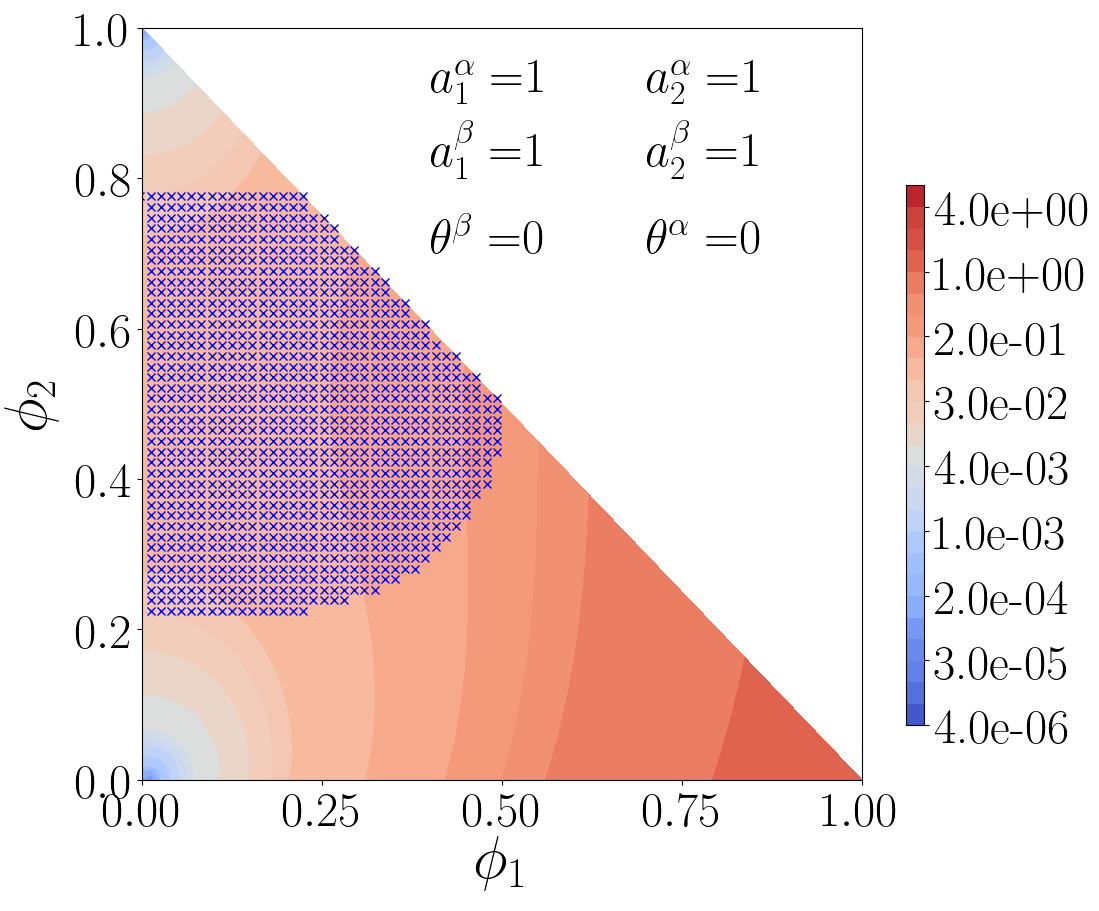
\includegraphics[width=0.6\linewidth]{figure/landscape}
	\caption{Exemple de paysage thermodynamique, la zone bleu représente la zone instable}
	\label{fig:landscape}
\end{figure}
%Les éléments de calculs pour la détermination de la zone instable sont présentés en annexe \ref{ann:stabphase}, cette zone correspond à des compositions pour lesquels le système subit une séparation de phase, ainsi il est primordiale que cette zone n'englobe pas les conditions initiales. Une représentation dans le plan est possible pour le cas ternaire, pour les cas comprenant un nombre plus important de paramètres d'ordre la visualisation semble plus complexe. Ainsi cette formulation possède l'avantage d'éviter un couplage entre le code CFD et un solveur d'équilibre thermodynamique (Open-Calphad par exemple) réduisant significativement le temps de développement. En effet pour les cas ou le paysage est connu il est alors possible de calibrer les paramètres des paraboloïdes pour obtenir une forme analytique proche du paysage réel. Dans le cas d'un paysage inconnu, par manque d'information thermodynamique, ce paysage permet d'avoir une description cohérente pour des simulations qualitatives.

La zone instable correspond à la zone où la séparation de phase a lieu, la détermination de cette zone est obtenue d'après \cite{aursand_spinodal_2017}. Une formulation analytique de cette forme permet d'éviter un couplage entre solveur d’équilibre thermodynamique (Open-Calphad par exemple) et le code CFD. Le temps de développement est alors fortement réduit. De plus, dans le cas d'un système sans données thermodynamiques, la formulation permet d'obtenir des simulations qualitatives. Dans le cas d'un système complètement décrit thermodynamiquement il suffit de trouver la formulation analytique qui convient (via un \textit{fit} par exemple). 


%On peut dès lors calculer le potentiel de diffusion homogène grâce à la formulation analytique (\ref{double_puit}) :
%\begin{align}
%	\tilde{\mu}_i & \nonumber= \frac{\partial}{\partial \phi_i}\left\lbrace 
%	\Omega^{\star} + \sum_j \tilde{\mu}_j^{eq}\phi_j + \left( {g}^{liq,eq} -  \sum_j \tilde{\mu}_j^{eq}\phi_j^{eq} \right)\right\rbrace \\
%	&\nonumber = \frac{\partial \Omega^{\star}}{\partial \phi_i} + \frac{\partial g^{liq,eq}}{\partial \phi_i} + \sum_j \frac{\partial \tilde{\mu}_j^{eq}\left(\phi_j - \phi_j^{eq}\right)}{\partial  \phi_i}\\
%	\tilde{\mu}_i &=	P^{dis}\frac{\partial P^{cont}}{\partial \phi_i} + P^{cont}\frac{\partial P^{dis}}{\partial \phi_i} + \tilde{\mu}_i^{eq}
%\end{align} 
%%\begin{align*}
%	%& \frac{\partial g^{liq,eq}}{\partial \phi_i} = 0 \\
%		%& \sum_j \frac{\partial \tilde{\mu}_j^{eq}\left(\phi_j - %\phi_j^{eq}\right)}{\partial  \phi_i} = \tilde{\mu}_i^{eq} %+\tilde{\mu}_{j\neq i}^{eq} \frac{\partial \phi_{j\neq i}}{\partial %\phi_i} = \tilde{\mu}_i^{eq}
%%\end{align*}
%L'objectif est alors de déterminer les paramètres des paraboloïdes pour obtenir des résultats consistants thermodynamiquement.



\chapter{Comparaison avec un cas de la littérature}
L'objectif de cette partie est de comparer les résultats obtenus par TrioCFD avec ceux présentés par Rao et al. \cite{rao_influence_2015}. Dans leur article Rao et al. présentent une expérience ainsi qu'un modèle CFD associé à l'experience permettant de modéliser le transfert de masse pour un cas ternaire.
\section{Présentation du cas de référence}
L'objectif de l'expérience est de visualiser la diffusion dans de l'eau de l'acétonitrile (miscible) contenue initialement dans une goutte composée également de chlorobenzène (non miscible). Ainsi à l'instant initial une goutte contenant un mélange d'acétonitrile et de chlorobenzène est formée, cette dernière étant plus légère que l'eau dans laquelle elle se trouve va commencer à monter, puis sous l'effet de la diffusion massique un changement de rapport de densité va subvenir et la goutte va redescendre.  
\begin{figure}[H]
	\centering
	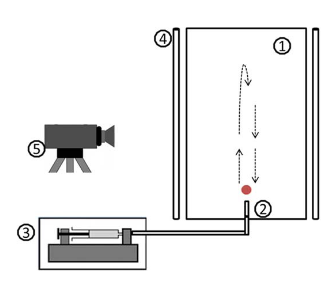
\includegraphics[width=0.3\linewidth]{figure/exp}
	\caption{Schéma de l'expérience, d'après \cite{rao_influence_2015}}
	\label{fig:exp}
\end{figure}
L'article présente également un modèle CFD, dans celui-ci le transfert de masse est calculé semi-empiriquement, à chaque itération la position de la goutte obtenue numériquement est comparée à la position obtenue expérimentalement, puis une régulation est mise en place pour déterminer un coefficient de transfert de masse via des corrélations pour faire diminuer cet écart, le ”modèle” alors obtenu n’est pas prédictible et une expérience physique est toujours nécessaire pour réaliser une simulation. L'algorithme est présenté en figure \ref{fig:algoRao}, 
\begin{figure}[H]
	\centering
	\begin{tikzpicture}[scale=0.75, transform shape]
	\node[draw,aspect=1.3, text centered,text width=3cm] (V) at (0,2.3) {Solution initiale };
	\node[draw,aspect=1.3, text centered,text width=2cm] (T) at (0,1.3) {$n=n+1$ };
	\node[draw,rectangle, text centered,minimum width=2cm,minimum height=1cm] (A)at(0,0){Estimation du transfert de masse à partir de corrélations};
	\node[draw,text centered,minimum width=2cm,minimum height=1cm] (B) at (0,-1.5) {Résolution des équations de Navier-Stokes};
	\node[draw,text centered,text width=10cm,minimum height=1cm] (C) at (0,-3) {Comparaison entre l'altitude de la goutte obtenue par CFD avec l'expérience, res = $f(z_{\text{CFD}},z_{\text{exp}})$};
	\node[draw,rectangle,diamond, aspect=1.3, text centered,text width=1.5cm] (D) at (0,-5) {res $<\varepsilon$ ? };
	
	\node[draw,rectangle,diamond, aspect=1.3, text centered,text width=1.5cm] (E) at (0,-7.3
	) { $t^{f}<t^{n}$ ? };
	\node[draw,aspect=1.3, text centered,text width=1.5cm] (W) at (0,-9) {Fin};
	%\node[draw,text centered,text width=2cm,minimum height=1cm] (E) at (0,-6.8) { $t=t^{n+1}$};
	%\node[draw,text centered,text width=7cm,minimum height=1cm] (Z) at (0,-6.2) { dsq}
	
	\node[draw,rectangle,diamond, aspect=1.3, text centered,text width=1cm,color=white] (H)at(-5,-5.9){ };
	\node[text centered,text width=1cm,color=black] (K1)at(0.5,-5.9){oui};
	\node[text centered,text width=1cm,color=black] (K2)at(-1.5,-4.8){non};
	\node[text centered,text width=1cm,color=black] (K3)at(0.5,-8.3){oui};
	\node[text centered,text width=1cm,color=black] (K4)at(-1.5,-7){non};
	%\node[draw,rectangle, text centered,diamond, aspect=1.3, text centered,text width=1cm] (I)at(6,-6){i=1 to n-1};
	\draw[->] (T.south) -- (A.north);
	\draw[->] (A.south) -- (B.north);
	\draw[->] (B.south) -- (C.north);
	\draw[->] (C.south) -- (D.north);
	\draw[->] (D.south) -- (E.north);
	\draw[->] (V.south) -- (T.north);
	\draw[->] (E.south) -- (W.north);
	\draw[->] (-7,1.3) -- (T.west);
	
	
	
	\draw (D.west)-- (-6,-5);
	\draw (-6,-5)-- (-6.,0);
	%	\draw (F.west)-- (-6.,0);
	\draw[->] (-6.,0) -- (A.west);
	\draw[-] (E.west) -- (-7,-7.3);
	\draw[-] (-7,-7.3) -- (-7,1.3);
	%\draw (G.east)-| (I.south);
	%\draw[->] (I.north)|- (A.east);
	\end{tikzpicture}
	\caption{Algorithme de résolution développé par Rao et al.\cite{rao_influence_2015}}
	\label{fig:algoRao}
\end{figure}
\section{Simulation réalisées}
\subsection{Choix du paysage thermodynamique}
L'objectif est alors d'utiliser un paysage de ce type pour résoudre un problème donné, pour cela quelques règles sont à garder en tête pour le choix d'un paysage thermodynamique. Dans un premier temps il est essentiel que les conditions initiales ne soient pas incluse dans la lacune de miscibilité, ce qui entraînerait une séparation de phase immédiate, un exemple de paysage de ce type est donnée en figure \ref{fig:landscapebase} et les résultats sont présentés par la figure \ref{land_base_sep}, on y observe une séparation de phase dès les premiers instants du calcul .
 \begin{figure}[H]
 	\centering
 	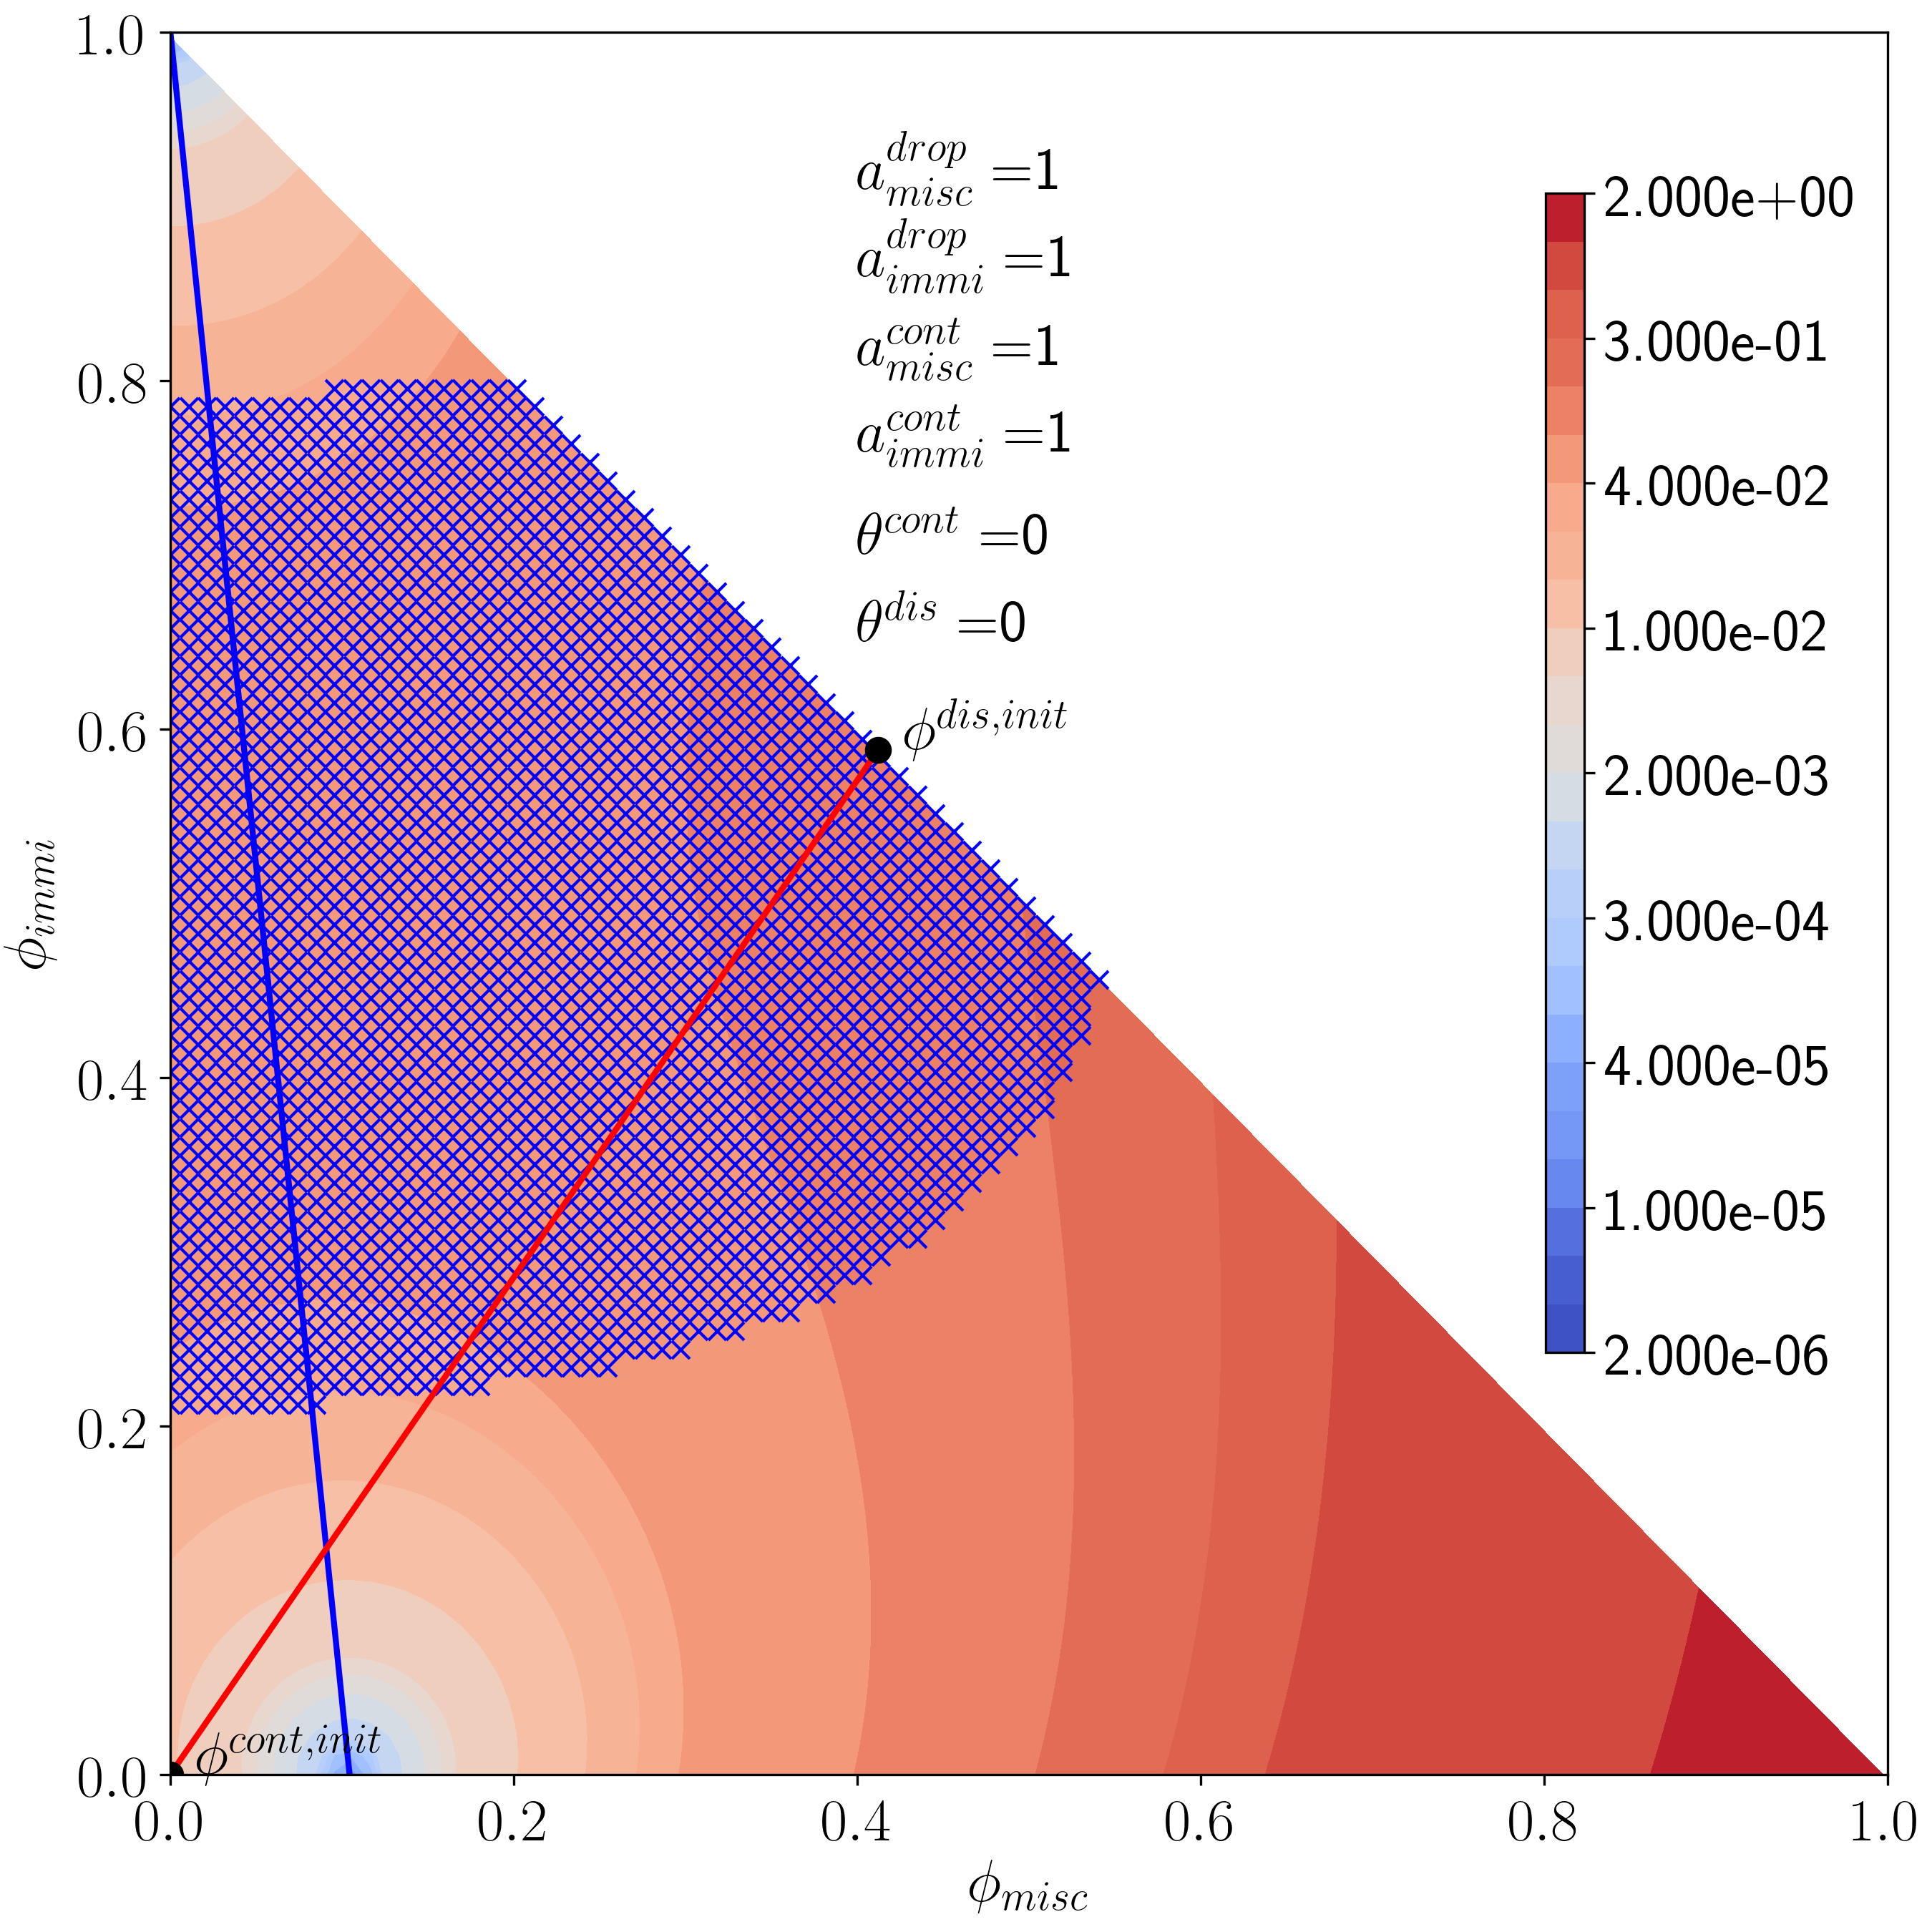
\includegraphics[width=0.4\linewidth]{figure/landscape_base.png}
 	\caption[Paysage thermodynamique]{Paysage thermodynamique, la droite bleu relie les deux  concentrations d'équilibre, la droite rouge relie les deux concentrations initiales}
 	\label{fig:landscapebase}
 \end{figure}
\vspace{-0.5cm}
 \begin{figure}[H]
 	\centering
 	\begin{subfigure}[H]{0.32\textwidth}
 		\centering
 		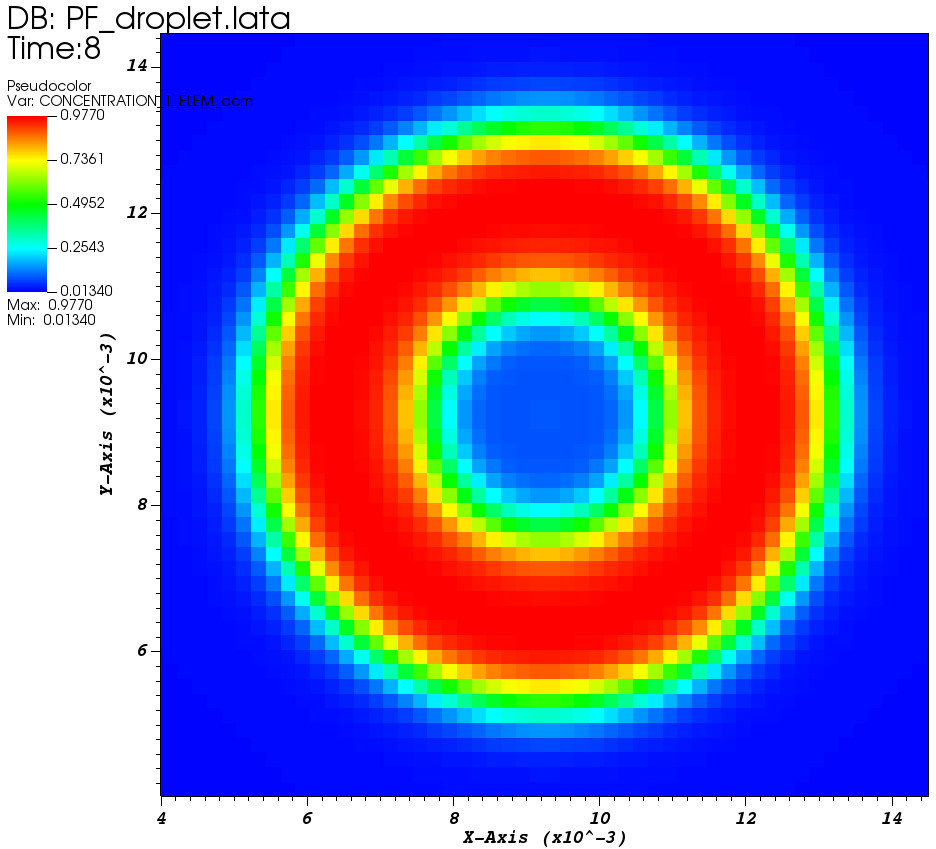
\includegraphics[width=\textwidth]{figure/paysage_base/visit0000.png}
 		\caption{Concentration immiscible}
 		\label{fig:y equals x}
 	\end{subfigure}
 	\begin{subfigure}[H]{0.32\textwidth}
 		\centering
 		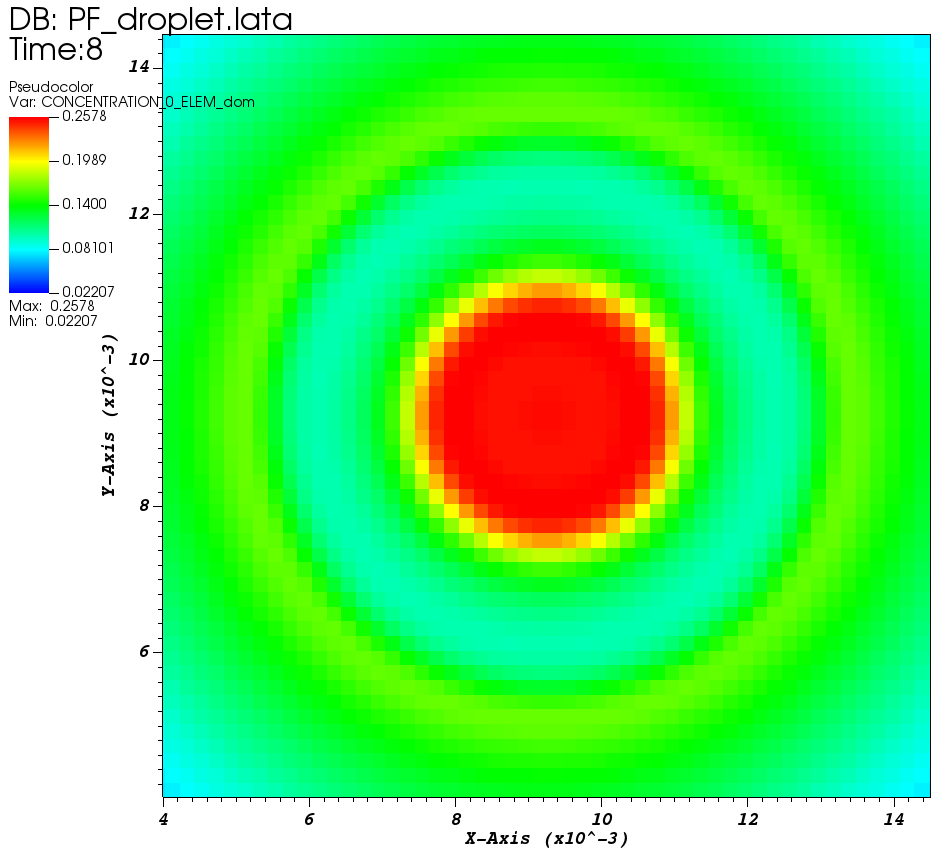
\includegraphics[width=\textwidth]{figure/paysage_base/visit0001.png}
 		\caption{Concentration miscible}
 		\label{fig:y equals x}
 	\end{subfigure}
 	\begin{subfigure}[H]{0.32\textwidth}
 		\centering
 		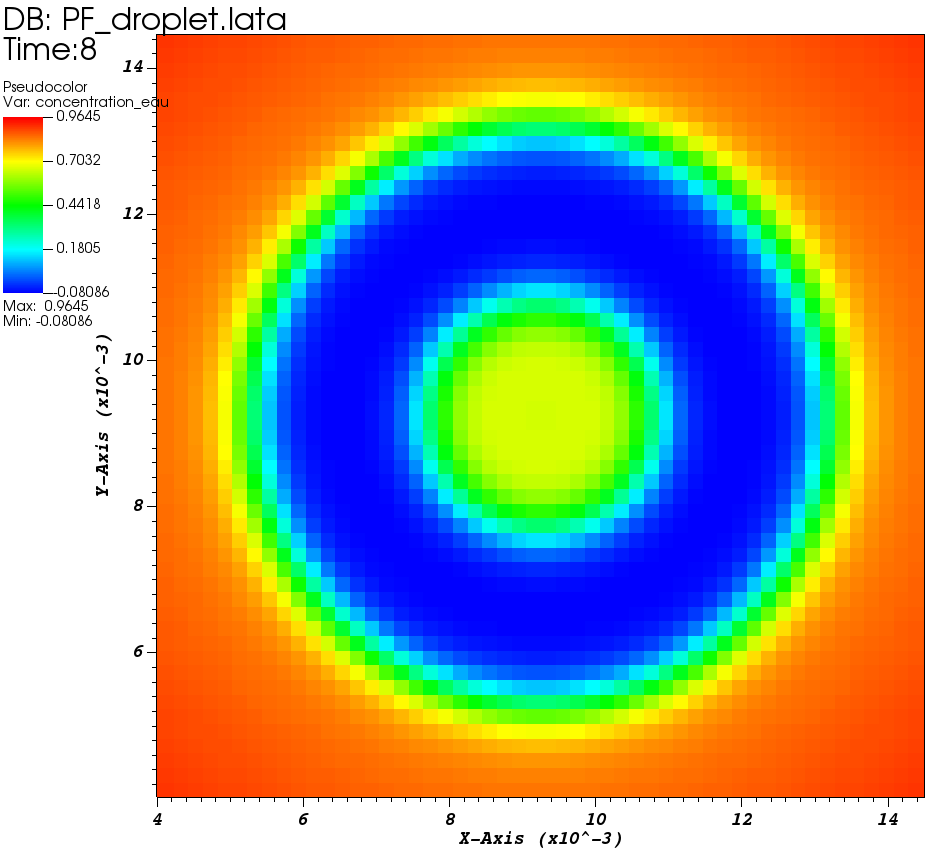
\includegraphics[width=\textwidth]{figure/paysage_base/visit0002.png}
 		\caption{Concentration eau}
 		\label{fig:y equals x}
 	\end{subfigure}
 	\caption{Séparation de phase dans la goutte}
 	\label{land_base_sep}
 \end{figure} \vspace{-0.5cm}
Sur la figure \ref{land_base_sep} on observe la présence de deux phases à l'intérieur de la goutte, une première uniquement composée de l'élément immiscible et la seconde composée d'eau et de l'élément miscible. On présente un deuxième paysage en figure \ref{fig:paysage2}
Comme expliqué précédemment ce paysage représente l'énergie libre volumique liée à l'équilibre des phases, ainsi on cherche à ce que les conditions initiales (ici aux extrémités de la droite rouge) soit hors de la zone instable et que la composition d'équilibre globale (placé a l'intersection des droites bleu et rouge) soit placée dans la lacune de miscibilité. Ainsi ce paysage semble correspondre parfaitement à ces deux critères. On souhaite également limiter l'entrée d'eau dans la goutte en régime transitoire, cette condition ce traduit par égalité entre la somme des deux compositions et l'unité. Hors ici le gradient d'énergie favorise un "chemin" différent. Pour vérifier cette présence d'eau, on considère alors un calcul statique (sans résolution des équations de Navier-Stokes) et on trace les concentrations à différents instants. On observe dès lors une importante intrusion d'eau dans la goutte dès les premiers instants, puis une séparation de phase est observable à l'intérieur de la goutte, phénomène que l'on souhaite absolument éviter.
 \begin{figure}[H]
 	\centering
 	\begin{subfigure}[H]{0.45\textwidth}
 		\centering
 		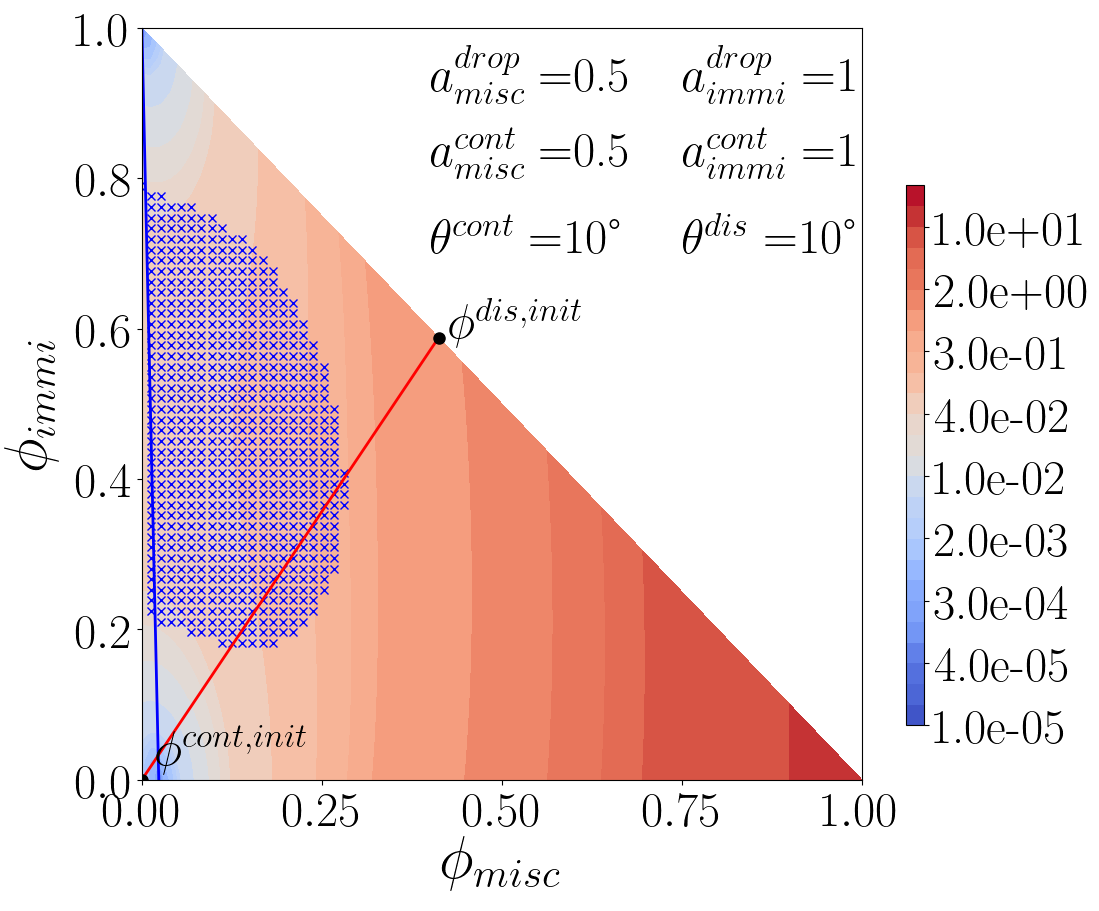
\includegraphics[width=\textwidth]{figure/paysage_neqlocal}
 		\caption{Paysage thermodynamique complet}
 		\label{fig:y equals x}
 	\end{subfigure}
 	\hfill
 	\begin{subfigure}[H]{0.45\textwidth}
 		\centering
 		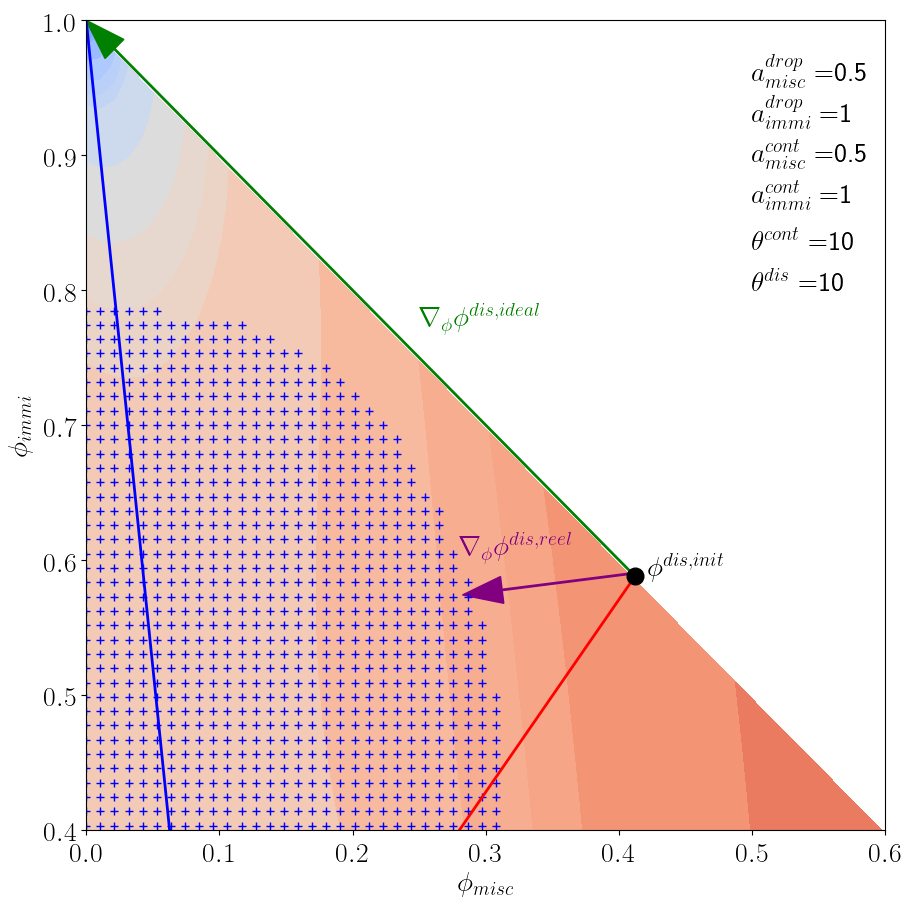
\includegraphics[width=\textwidth]{figure/direction_gradient}
 		\caption{Paysage thermodynamique partiel}
 		\label{fig:y equals x}
 	\end{subfigure}
 	\caption{Paysage thermodynamique et direction privilégiée par le système, la flèche verte représente le cas idéal sans intrusion d'eau et la flèche violette le cas associé au paysage thermodynamique, la zone bleu correspond à la zone instable}
 	\label{fig:paysage2}
 \end{figure}\vspace{-0.9cm}
 \begin{figure}[H]
 	\centering
 	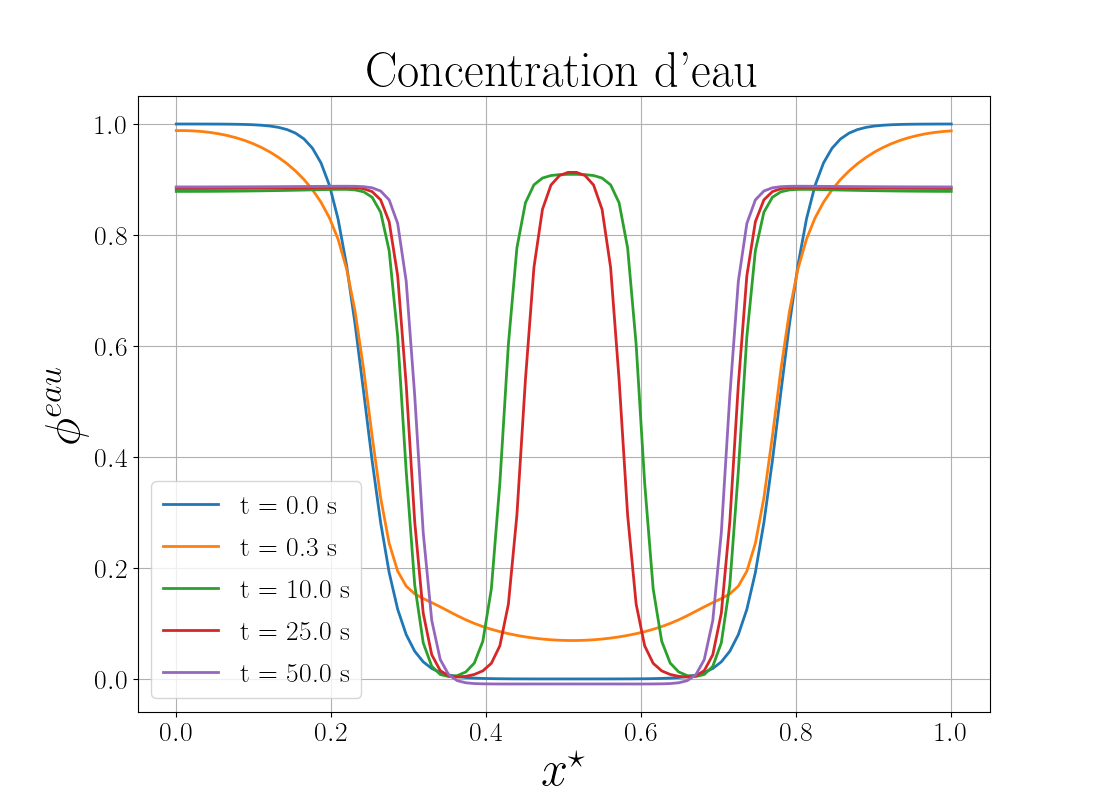
\includegraphics[width=0.7\linewidth]{figure/eau_ref}
 	\caption[Concentration d'eau dans le domaine]{Concentration d'eau dans le domaine, $x^{\star} = x / L_x$ représente une longueur adimensionnée}
 	\label{fig:eauref}
 \end{figure}\vspace{-0.7cm}
Finalement au travers de ces deux exemples, nous avons montré que pour qu'un paysage soit cohérent et potentiellement utilisable certaines conditions sont à remplir. Les critères concerne la position des conditions initiales, qui doivent être en dehors de la zone instable, un second critère concerne l'absence nécessaire de la zone instable sur le "chemin" de chacune des phases et finalement une direction initiale privilégiant une imperméabilité à l'eau dans la goutte.
\subsection{Validation d'un paysage}
Dans la suite on utilisera le paysage présenté en figure \ref{fig:thechoosenone} répondant à l'ensemble de ces critères.
\begin{figure}[H]
		\centering
		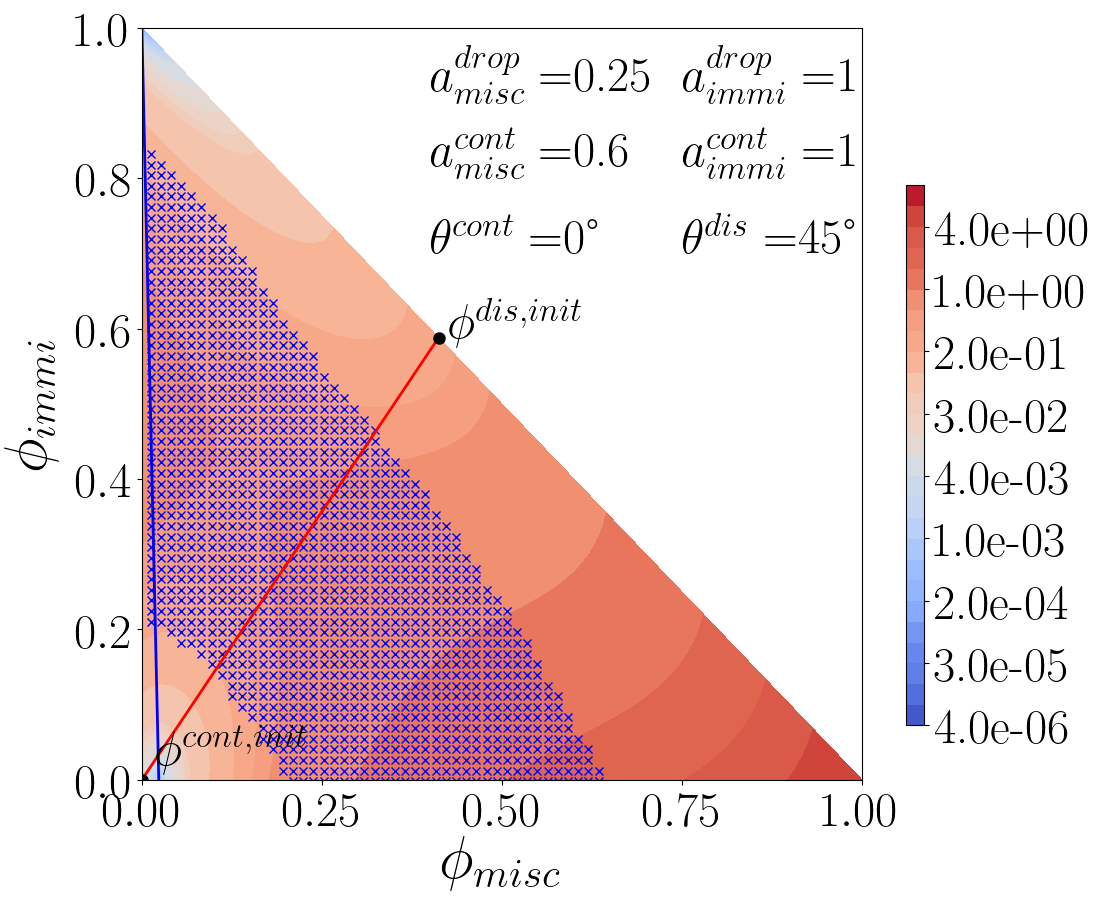
\includegraphics[width=0.45\textwidth]{figure/Paysage_ecriture1.png}
	\caption{Paysage thermodynamique choisit pour la simulation}
	\label{fig:thechoosenone}
\end{figure}

On cherche à tracer la solution stationnaire, sans couplage avec les équations de Navier-Stokes, on observe alors une non-monotonie de l'interface pour le composant miscible, de plus à l'intérieur de la goutte la concentration de composant miscible est négative et la composition d'élément immiscible est quant à elle supérieure à 1, de façon à obtenir une somme des deux concentrations égale à l'unité.
\begin{figure}[H]
	\centering
	\begin{subfigure}[H]{0.45\textwidth}
		\centering
		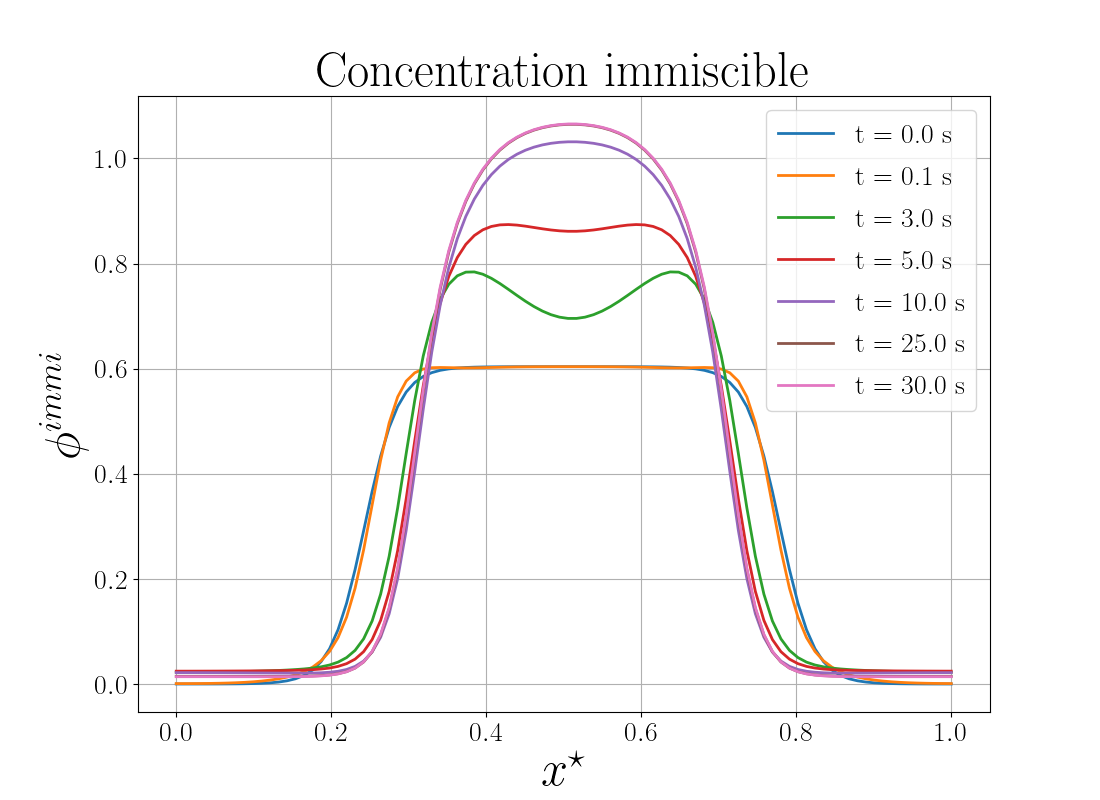
\includegraphics[width=\textwidth]{figure/nouveau_parametrage/immiscible_New_Parametrage.png}
		\caption{Concentration immiscible}
		\label{fig:y equals x}
	\end{subfigure}
	\hfill
	\begin{subfigure}[H]{0.45\textwidth}
		\centering
		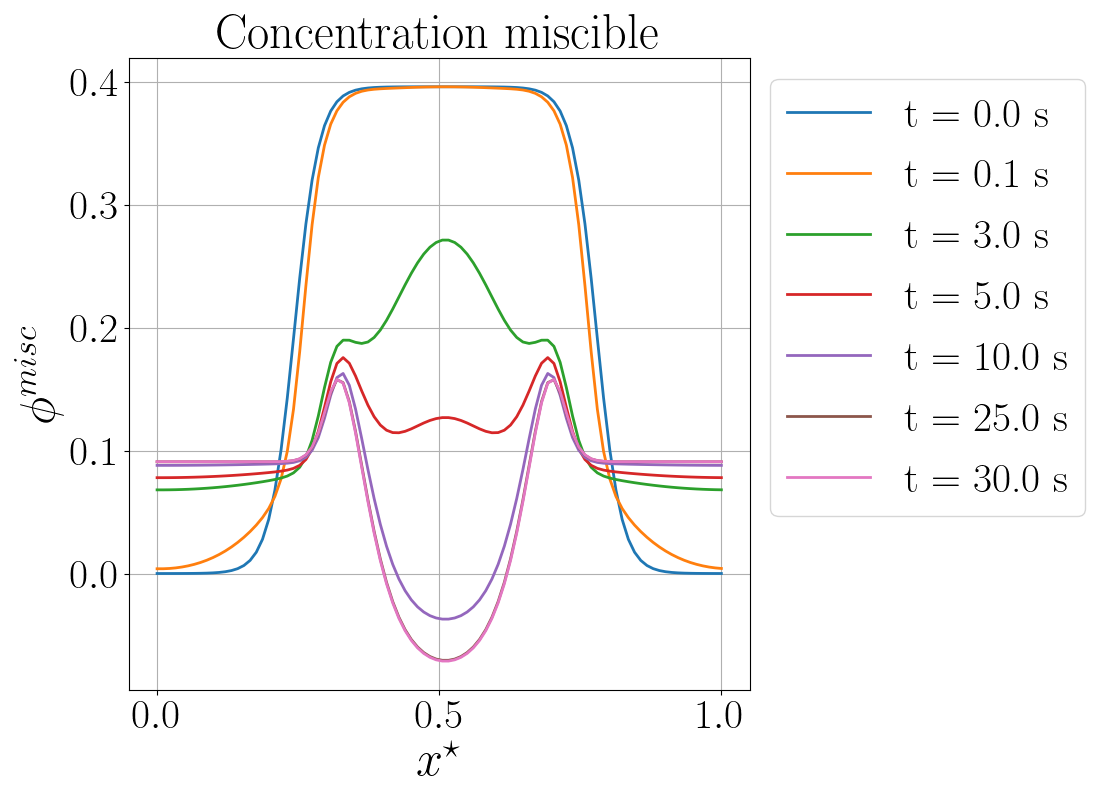
\includegraphics[width=\textwidth]{figure/nouveau_parametrage/miscible_New_Parametrage.png}
		\caption{Concentration miscible}
		\label{fig:y equals x}
	\end{subfigure}
\end{figure} \vspace{-0.8cm}
\begin{figure}[H]
	\centering
	\ContinuedFloat
	\begin{subfigure}[H]{0.45\textwidth}
		\centering
		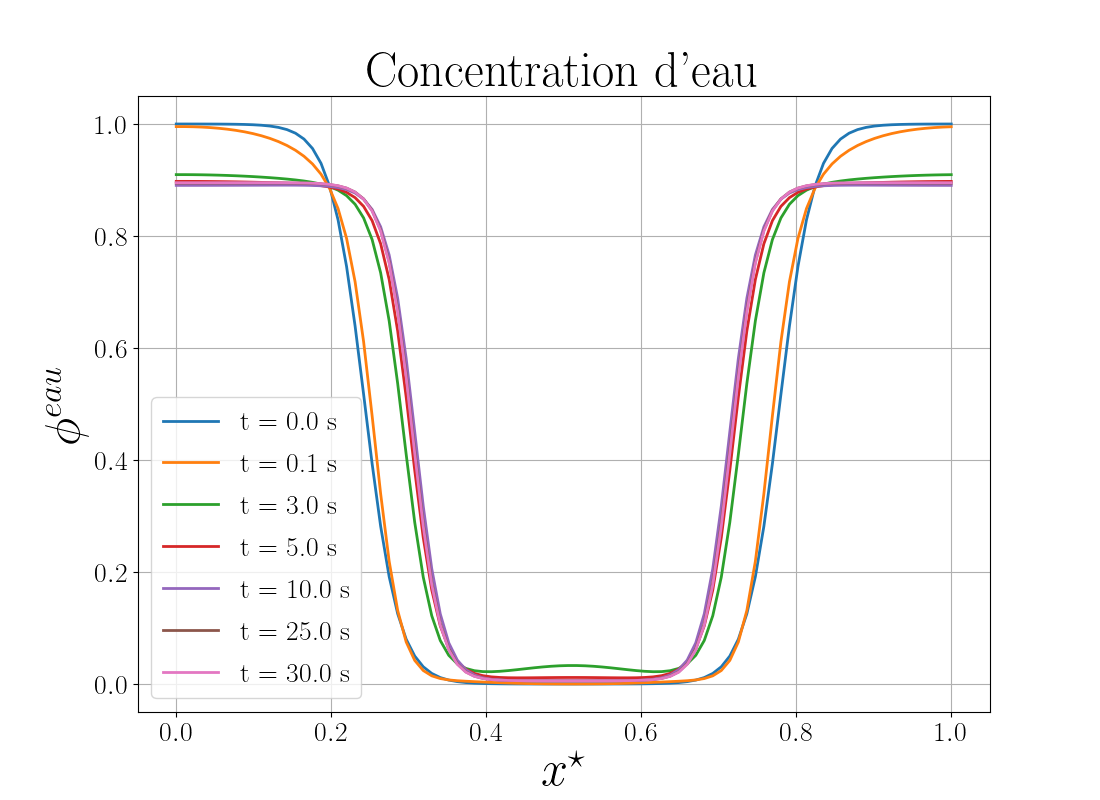
\includegraphics[width=\textwidth]{figure/nouveau_parametrage/eau_New_Parametrage.png}
		\caption{Concentration d'eau}
	\end{subfigure}
	\caption{Variation de la concentration des différents composants au cours du temps}
\end{figure}
On remarque alors une non-monotonie de l'interface. L'article \cite{rasolofomanana_diffuse-interface_2022} présente un paramétrisation du coefficient de gradient pour traiter les non monotonie d'interface, cette paramétrisation utilise la symétrie de la matrice coefficient de gradient pour la réécrire sous la forme :
\begin{equation}
\bar{\bar{\bm{\kappa}}} = \alpha \bm{R}\bm{D}\bm{R}^T
\label{eq:param_kappa}
\end{equation}
avec : $\bm{R}$ une matrice de rotation et $\bm{D}$ une matrice diagonale de la forme :
\begin{equation}
\bm{R} =    \begin{pmatrix} 
\cos\varphi & -\sin\varphi \\ 
\sin\varphi				&  \cos\varphi
\end{pmatrix}
\end{equation}
\begin{equation}
	\bm{D}(d) =    \begin{pmatrix} 
	2 & 0 \\ 
	0 & d
	\end{pmatrix} 
\end{equation}
La cohérence avec le système binaire est assurée par le coefficient $\alpha$ obtenu tel que :
\begin{equation}
\alpha = \frac{\kappa^{bin}}{2\cos^2\varphi + d \sin^2\varphi}
\end{equation}
On présente les différents résultats issus de la paramétrisation du coefficient de gradient : 
\begin{figure}[H]
		\centering
		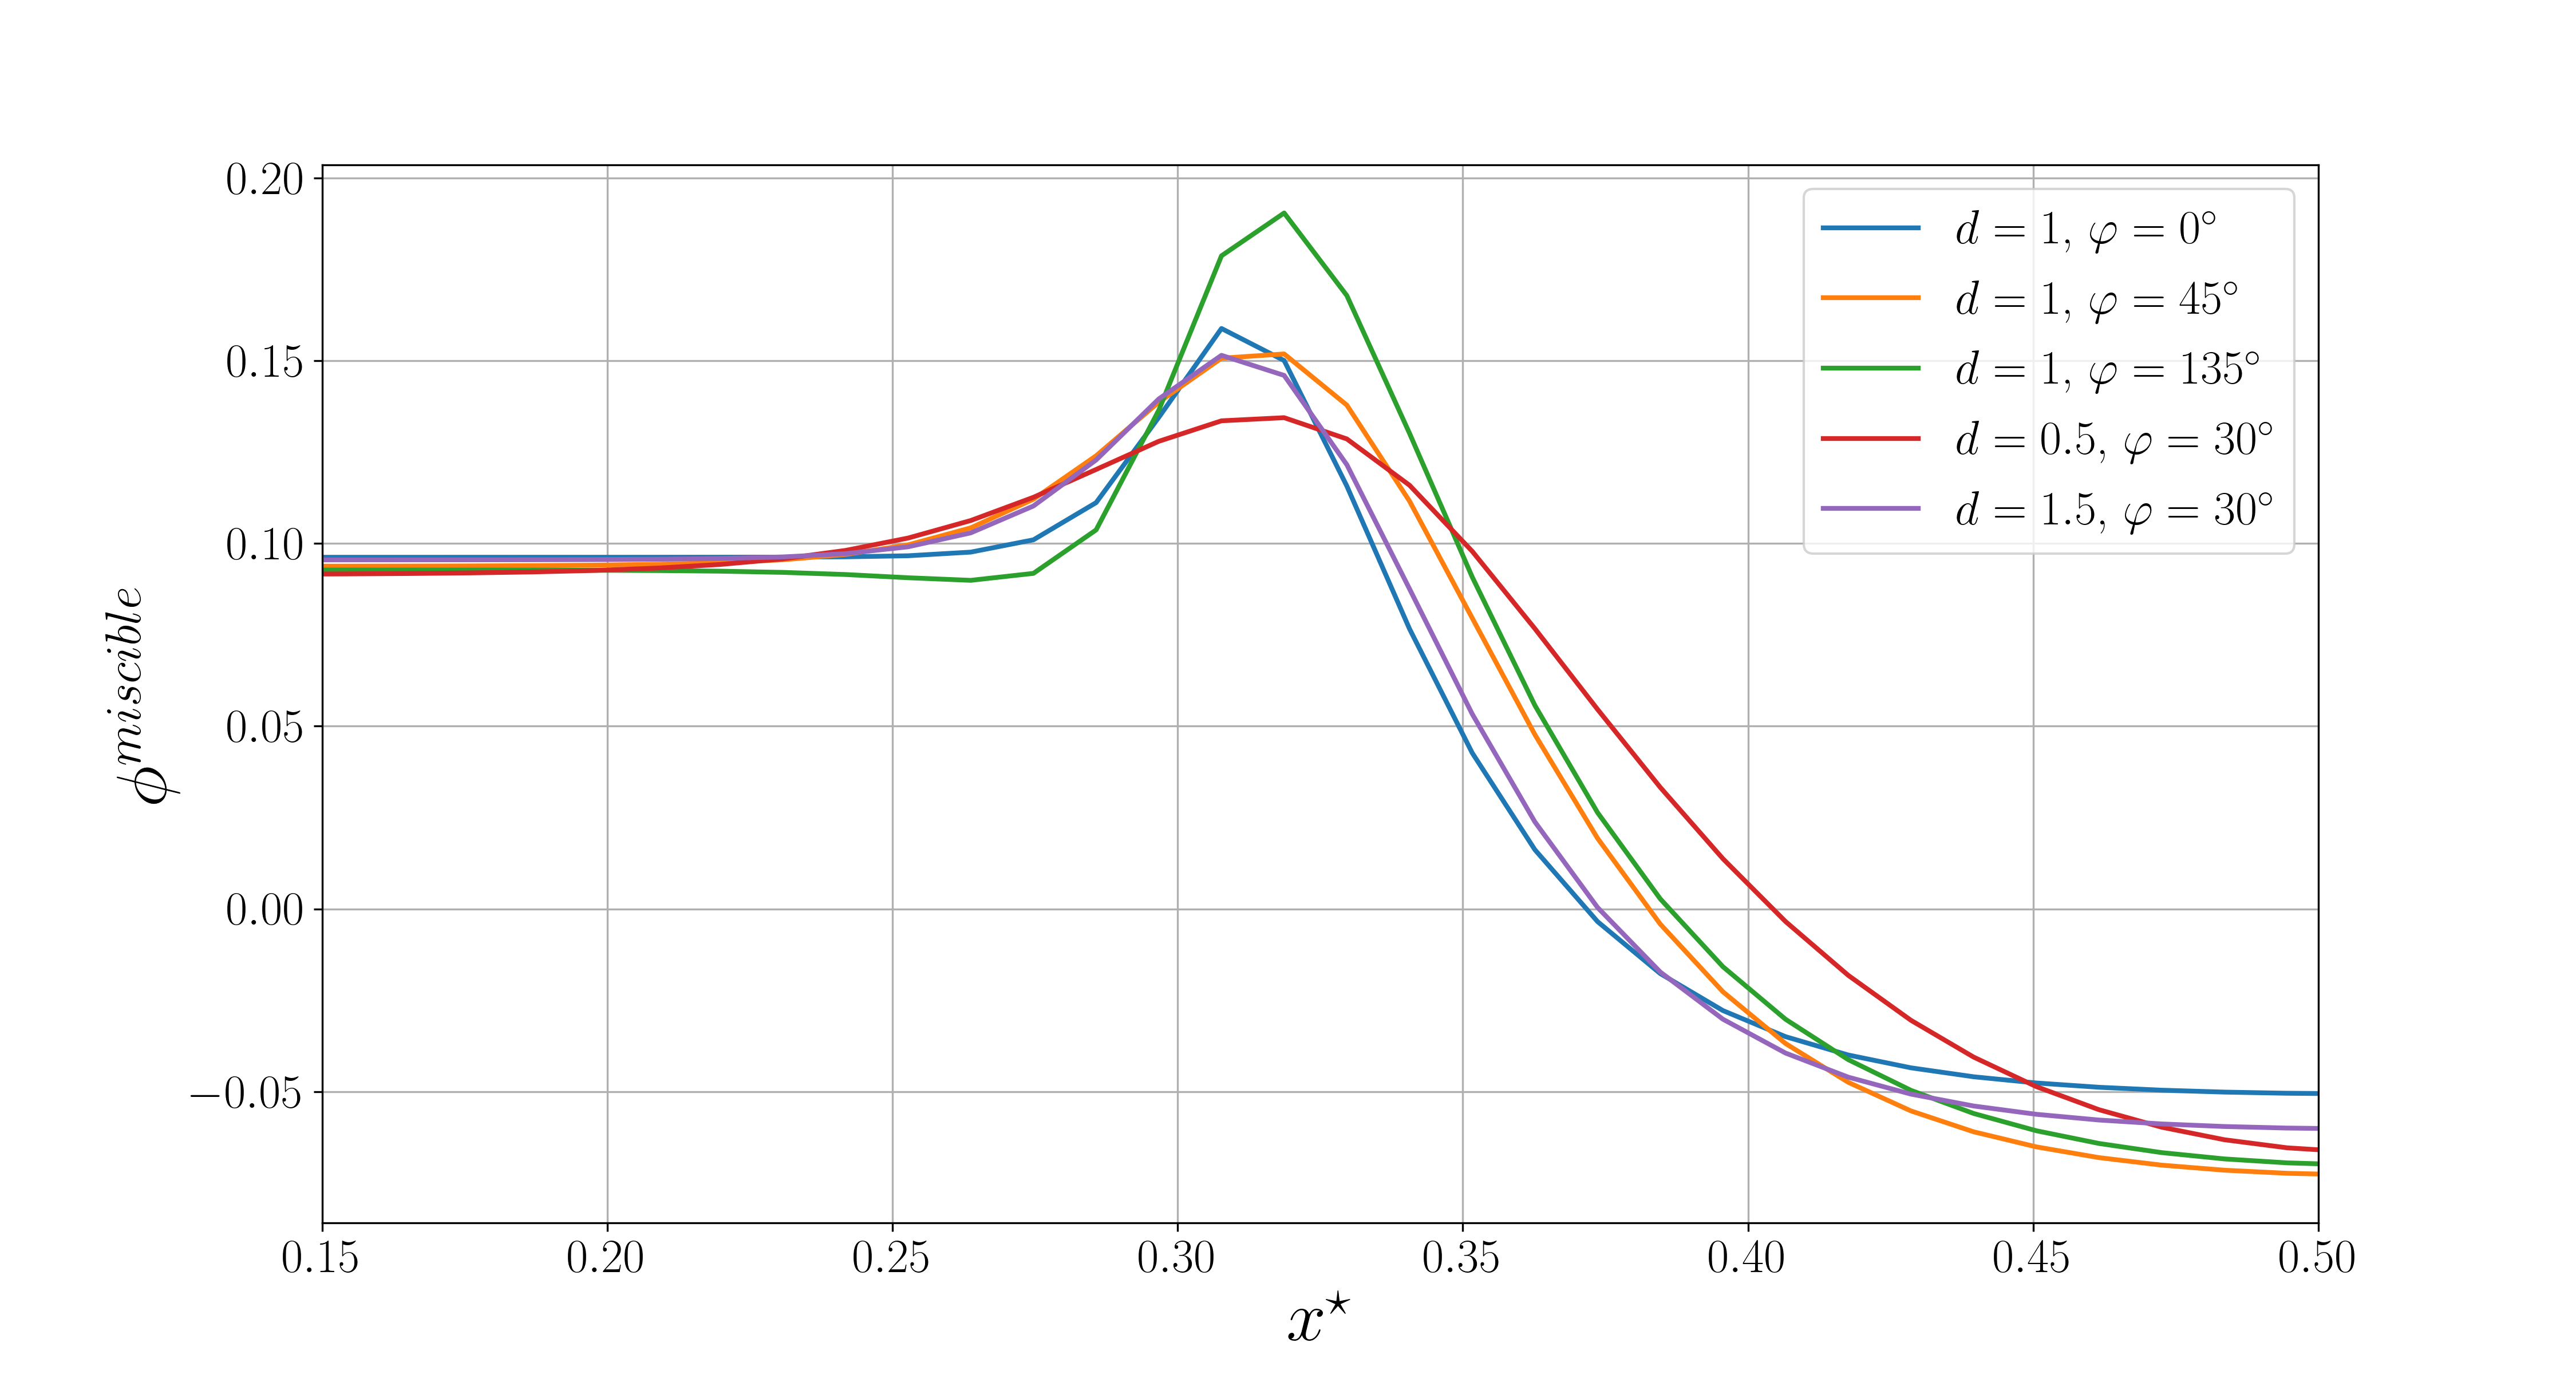
\includegraphics[width=0.7\textwidth]{figure/ProfInterfStatio2.png}
		\caption{Profils de l'interface pour différents paramétrages du coefficient de gradient}
\end{figure}


% ======================================== Fin Document ========================================

% ======================================== Début Listes & Co ========================================

\begin{figure}[H]
	\centering
	\begin{tikzpicture}
	\node[draw,aspect=1.3, text centered,text width=3cm] (V) at (0,2.3) {Solution initiale };
	\node[draw,aspect=1.3, text centered,text width=2cm] (T) at (0,1.3) {$n=n+1$ };
	\node[draw,rectangle, text centered,minimum width=2cm,minimum height=1cm] (A)at(0,0){Estimation du transfert de masse à partir de corrélations};
	\node[draw,text centered,minimum width=2cm,minimum height=1cm] (B) at (0,-1.5) {Résolution des équations de Navier-Stokes};
	\node[draw,text centered,text width=10cm,minimum height=1cm] (C) at (0,-3) {Comparaison entre l'altitude de la goutte obtenue par CFD avec l'expérience, res = $f(z_{\text{CFD}},z_{\text{exp}})$};
	\node[draw,rectangle,diamond, aspect=1.3, text centered,text width=1.5cm] (D) at (0,-5) {res $<\varepsilon$ ? };

	\node[draw,rectangle,diamond, aspect=1.3, text centered,text width=1.5cm] (E) at (0,-7.3
	) { $t^{f}<t^{n}$ ? };
	\node[draw,aspect=1.3, text centered,text width=1.5cm] (W) at (0,-9) {Fin};
	%\node[draw,text centered,text width=2cm,minimum height=1cm] (E) at (0,-6.8) { $t=t^{n+1}$};
	%\node[draw,text centered,text width=7cm,minimum height=1cm] (Z) at (0,-6.2) { dsq}
	
	\node[draw,rectangle,diamond, aspect=1.3, text centered,text width=1cm,color=white] (H)at(-5,-5.9){ };
	\node[text centered,text width=1cm,color=black] (K1)at(0.5,-5.9){oui};
	\node[text centered,text width=1cm,color=black] (K2)at(-1.5,-4.8){non};
	\node[text centered,text width=1cm,color=black] (K3)at(0.5,-8.3){oui};
	\node[text centered,text width=1cm,color=black] (K4)at(-1.5,-7){non};
	%\node[draw,rectangle, text centered,diamond, aspect=1.3, text centered,text width=1cm] (I)at(6,-6){i=1 to n-1};
	\draw[->] (T.south) -- (A.north);
	\draw[->] (A.south) -- (B.north);
	\draw[->] (B.south) -- (C.north);
	\draw[->] (C.south) -- (D.north);
	\draw[->] (D.south) -- (E.north);
	\draw[->] (V.south) -- (T.north);
	\draw[->] (E.south) -- (W.north);
	\draw[->] (-7,1.3) -- (T.west);
	
	
	
	\draw (D.west)-- (-6,-5);
	\draw (-6,-5)-- (-6.,0);
%	\draw (F.west)-- (-6.,0);
	\draw[->] (-6.,0) -- (A.west);
	\draw[-] (E.west) -- (-7,-7.3);
	\draw[-] (-7,-7.3) -- (-7,1.3);
	%\draw (G.east)-| (I.south);
	%\draw[->] (I.north)|- (A.east);
	
	\end{tikzpicture}
	\caption{Algorithme de résolution développé par Rao et al.\cite{rao_influence_2015}}
\end{figure}

\newpage
\printbibliography
\appendix

\chapter{Solution analytique pour une interface plane}
La solution analytique stationnaire permet de donner des conditions initiales cohérentes, ainsi on s'intéresse au cas binaire "classique" (avec un seul paramètre d'ordre noté $\phi$) avec des points d'équilibres placés aux extremums, le composé est choisi comme complètement miscible. La densité d'énergie est alors choisit sous une forme analytique polynomiale d'ordre 4 en double puits :
\begin{equation}
	f(\phi) = \phi^2 (1-\phi)^2
	\label{eq:anal_bin}
\end{equation}
On rappel fonctionnelle de Ginzburg-Landau :
\begin{equation}
	\mathbb{F} =\int_V \lambda f(\phi) + \frac{1}{2}\kappa ||\nabla \phi||^2 dV
\end{equation}
Avec $\lambda$ un paramètre d'upscalling présenté précédemment, $\kappa$ un coefficient de gradient.
La condition d'équilibre est définit tel que :
\begin{equation}
	\kappa \frac{d^2\phi}{dz^2} = \lambda \frac{d f(\phi)}{d\phi}
\end{equation}
L'astuce consiste alors par multiplier l'équation par $\displaystyle \frac{d\phi}{dz}$ puis d'intégrer entre 0 et $z$, soit :
\begin{align}
	& \kappa \frac{d^2\phi}{dz^2}\frac{d\phi}{dz} = \lambda \frac{d f(\phi)}{d\phi}\frac{d\phi}{dz} \\
	\Rightarrow & \kappa \int_0^z \frac{d^2\phi}{dz^2}\frac{d\phi}{dz} dz= \int_0^z \frac{d f(\phi)}{dz} dz
\end{align}
Loin de l'interface, en $z=0$ on considère le système à l'équilibre soit $\frac{d\phi}{dz} = 0$ et on fixe une condition au limite de type Dirichlet homogène :
\begin{equation}
	\phi (z= 0) = 0 \Rightarrow f(0) = 0
\end{equation}
Finalement le résultat de l'intégration précédente nous donne :
\begin{equation}
		\cfrac{\kappa}{2} \frac{d\phi}{dz} = \lambda f(\phi)
\end{equation}
En remplaçant $f(\phi)$ par sa formulation analytique \ref{eq:anal_bin} : 
\begin{equation}
	\frac{d\phi}{\phi(1-\phi)} = \sqrt{\frac{2\lambda}{\kappa}} dz
	\label{solution_statio_plane}
\end{equation}
En posant $u = 2\phi - 1$ soit $du = 2d\phi$
\begin{align*}
	 \cfrac{d\phi}{\phi(1-\phi)} &= \cfrac{\cfrac{du}{2}}{\left(\cfrac{u+1}{2}\right)\left( 1 -\cfrac{u+1}{2}\right)} \\
	 & = \frac{2du}{(1+u)(1-u)} \\
	 & = 2\frac{du}{1-u^2}
\end{align*}
Finalement l'équation \ref{solution_statio_plane} devient :
\begin{equation}
	\frac{du}{1-u^2} = \cfrac{1}{2}\sqrt{\frac{2\lambda}{\kappa}}dz
\end{equation}
On remarque que le termes de gauche correspond à la dérivée de la fonction réciproque de la tangente hyperbolique, soit :
\begin{equation}
	\text{arctanh}(u) = \cfrac{1}{2}\sqrt{\frac{2\lambda}{\kappa}} z + C
\end{equation}
Avec $C$ une constante d'intégration.
En réutilisant le changement de variable il est immédiat que :
 \begin{equation}
 \phi(z) = \frac{1}{2}\left(\tanh \left(\cfrac{1}{2}\sqrt{\frac{2\lambda}{\kappa}}z +C\right)+1\right)
 \end{equation}
La constante $C$ peut être déterminé à partir d'une valeur moyenne du paramètre d'ordre, cette résolution ne sera pas explicité ici.

\section{Méthode de calcul}






\chapter{De la tension de surface au coefficients de gradient}
\section{Méthode générale}
Cette deuxième annexe présente la méthode de calcul des coefficients de gradient à partir de la tension de surface qui est une donnée physique du système. Physiquement la tension interfaciale $\sigma$ représente l'excès d'énergie libre par unité de surface associé à la présence d'une interface entre deux phases distinctes, on peut ainsi la écrire :
\begin{equation}
\sigma = \cfrac{\mathbb{F}-\mathbb{F}^{hom}}{S}
\end{equation}
Où $S$ représente la surface de l'interface, $\mathbb{F}$ l'énergie libre du système et $\mathbb{F}$ l'énergie libre homogène du système, c'est-à-dire l'énergie libre du système dénuée d'interface. 
Dans un premier temps on rappel la forme des fonctionnelles de Ginzburg-Landau associées à ses deux systèmes :
\begin{align*}
&\mathbb{F} = \int_{V}\sum_{i=1}^{n-1}\sum_{j=1}^{n-1}\frac{\kappa_{ij}}{2}\nabla \phi_i \cdot \nabla \phi_j + f(\phi_1,..,\phi_{n-1}) - \sum_{1}^{n-1}\tilde{\mu}_i^{eq}\phi_i dV \\
&\mathbb{F}^{hom} = \int_V f^{\alpha,eq}  - \sum_{1}^{n-1}\tilde{\mu}_i^{eq}\phi_i^{\alpha,eq} dV 
\end{align*}
Ainsi en combinant les deux équations précédentes : 
\begin{equation}
\sigma = \int_{V}\sum_{i=1}^{n-1}\sum_{j=1}^{n-1}\frac{\kappa_{ij}}{2}\nabla \phi_i \cdot \nabla \phi_j + f(\phi_1,..,\phi_{n-1}) - f^{\alpha,eq} - \sum_{1}^{n-1}\tilde{\mu}_i^{eq}(\phi_i-\phi_i^{\alpha,eq}) dV
\end{equation}
Dans le cas 1D suivant $z$ l'équation précédente devient : 
\begin{equation}
\sigma = \int_{0}^L\sum_{i=1}^{n-1}\sum_{j=1}^{n-1}\frac{\kappa_{ij}}{2}\frac{ d\phi_i}{dz} \frac{ d\phi_j}{dz} + f(\phi_1,..,\phi_{n-1}) - f^{\alpha,eq} - \sum_{1}^{n-1}\tilde{\mu}_i^{eq}(\phi_i-\phi_i^{\alpha,eq}) dz
\end{equation}
La condition d'équilibre s'écrit :
\begin{equation}
\sum_{j=1}^{n-1} \kappa_{i,j} \frac{d^2\phi_j}{dz^2} = \left.\frac{\partial f}{\partial \phi_i}\right|_{\phi_{j\neq i}} - \tilde{\mu}_i^{eq}
\end{equation}
Après multiplication par $\displaystyle \frac{d\phi_i}{dz}$ et intégration on trouve :
\begin{equation}
\sigma = \int_0^L \sum_{i=1}^{n-1}\sum_{j=1}^{n-1} \kappa_{i,j}\frac{d\phi_i}{dz}\frac{d\phi_j}{dz}dz
\end{equation}
On retrouve alors la relation permettant la détermination de ce coefficient dans le cas binaire en posant $n=2$
\begin{equation}
\sigma = \int_0^L\kappa^{bin}\left(\frac{d\phi}{dz}\right)^2dz
\end{equation}
Sauf mention contraire, dans le cadre de l'étude on considère :
\begin{equation}
\bm{\bar{\bar{\kappa}}} =    \begin{pmatrix} 
\kappa^{bin}& 0 \\ 
0				& \kappa^{bin} 
\end{pmatrix} 
\end{equation}

\chapter{Séquence de dégradation du c\oe ur} \label{annexe:seq_deg}
D'après \cite{kolev_multiphase_2015} voici le scénario de fonte du c\oe ur :
\begin{itemize}
	\item[$\bullet$] \underline{Entre 800 et 900 \textdegree C :} L'augmentation de la pression à l'intérieur de la gaine en zirconium provoque un gonflement puis une rupture de cette dernière.
	\item[$\bullet$] \underline{Entre 900 et 1300 \textdegree C :} Début de la réaction fortement exothermique d'oxydation de la gaine. A cet instant une forte proportion de la puissance thermique dégagée provient de cette réaction. La molécule d'eau est dissociée, l'oxygène est absorbé par la surface métallique et l'hydrogène est libéré. L'absorption de l'hydrogène dans les fissures du métal le fragilise davantage et accélère le processus de défaillance de la gaine. De plus l'apparition de fissure augmente la surface de réaction provoquant une accélération de la réaction.
	\item[$\bullet$] \underline{Entre 1300 et 1400 \textdegree C :} Apparition d'alliages constitués des matériaux composant la gaine (principalement Zr) et de l'acier présent dans la cuve.
	\item[$\bullet$] \underline{Entre 1400 et 1500 \textdegree C :} Fusion et rupture des structures métallique du c\oe ur. Libération des composant en phase gazeuse du combustible.
	\item[$\bullet$] \underline{Entre 1500 et 1850 \textdegree C :} Point de fusion du zirconium, dissolution du dioxyde d'uranium UO$_2$ par le zirconium en fusion, apparition de l'alliage (U,O,Zr)
	\item[$\bullet$] \underline{Entre 2000 et 2650 \textdegree C :} Fusion du ZrO$_2$, dissolution de l'UO$_2$ dans le ZrO$_2$ fondu et formation de la solution liquide UO$_2$-ZrO$_2$.
\end{itemize}

\end{document}


\section{Évaluation des paraboloïdes}

L'objectif est de paramétrer les paraboloïdes afin d'obtenir des valeurs proches de la réalité. Malheureusement le trop grand nombre de paramètres, ne permettent pas la convergence des algorithmes de fit 'classique'. \\
Pour remédier à ce problème on découpe le problème en deux sous problèmes:
\begin{enumerate}
	\item On transforme le produit des deux paraboloïdes en un polynôme de degré 4 
	\item On résout un système liant les coefficients polynomiaux aux paramètres des paraboloïdes
\end{enumerate} 
Ainsi on exprime :
\begin{equation}
\Omega^{\star} = \sum_{i,j} c_{ij}\left.\phi^{misc}\right.^i\left.\phi^{immi}\right.^j
\end{equation}
On note alors $\bm{\Gamma} = \left.\phi^{misc}\right.^i\left.\phi^{immi}\right.^j $ la matrice contenant les variables du polynôme, $\bm{c} = c_{ij}$ le vecteur contenant les coefficient polynomiaux et $\bm{\Theta} $ le vecteur contenant les valeurs issus d'Open-CALPHAD. Ainsi on cherche à résoudre :
\begin{equation}
\bm{\Gamma c = \Theta}
\end{equation}
Or on a cond($\Gamma$)$ \simeq 20626\gg 1$ ainsi le problème est mal conditionné (sur-déterminé) et les résultats ne peuvent être satisfaisant.

\section{Solution analytique pour une interface plane}
La solution analytique stationnaire permet de donner des conditions initiales cohérentes, ainsi on s'intéresse au cas binaire "classique" (avec un seul paramètre d'ordre noté $\phi$), La densité d'énergie est choisit de la forme analytique d'ordre 4 en double puits :
\begin{equation}
f(\phi) = \phi^2 (1-\phi)^2
\end{equation}
La fonctionnelle de Ginzburg-Landau est alors de la forme :
\begin{equation}
\mathbb{F} =\int_V \lambda f(\phi) + \frac{1}{2}\kappa ||\nabla \phi||^2 dV
\end{equation}
Dans l'état stationnaire, la condition d'équilibre nous donne :
\begin{equation}
\kappa \frac{d^2\phi}{dz^2} = \lambda \frac{d f(\phi)}{d\phi}
\end{equation}
L'astuce est alors de multiplier l'équation par $\displaystyle \frac{d\phi}{dz}$ puis d'intégrer entre 0 et $L$, soit :
\begin{align}
& \kappa \frac{d^2\phi}{dz^2}\frac{d\phi}{dz} = \lambda \frac{d f(\phi)}{d\phi}\frac{d\phi}{dz} \\
\Rightarrow & \kappa \int_0^z \frac{d^2\phi}{dz^2}\frac{d\phi}{dz} dz= \int_0^z \frac{d f(\phi)}{dz} dz
\end{align}
Loin de l'interface, en $z=0$ on considère le système à l'équilibre soit $\frac{d\phi}{dz} = 0$ et on fixe une condition au limite de type Dirichlet homogène :
\begin{equation}
\phi (z= 0) = 0 \Rightarrow f(0) = 0
\end{equation}
Finalement le résultat de l'intégration précédente nous donne :
\begin{equation}
\frac{1}{2}\kappa \left(\frac{d\phi}{dz}\right) = \lambda f(\phi)
\end{equation}
En remplaçant $f(\phi)$ par sa formulation analytique : 
\begin{equation}
\frac{d\phi}{\phi(1-\phi)} = \sqrt{\frac{2\lambda}{\kappa}} dz
\label{solution_statio_plane}
\end{equation}
En posant $u = 2\phi - 1$ soit $du = 2d\phi$
\begin{align*}
\cfrac{d\phi}{\phi(1-\phi)} &= \cfrac{\cfrac{1}{2}du}{\left(\cfrac{u+1}{2}\right)\left( 1 -\cfrac{u+1}{2}\right)} \\
& = \frac{2du}{(1+u)(1-u)} \\
& = 2\frac{du}{1-u^2}
\end{align*}
Finalement l'équation \ref{solution_statio_plane} devient :
\begin{equation}
\frac{du}{1-u^2} = \cfrac{1}{2}\sqrt{\frac{2\lambda}{\kappa}}dz
\end{equation}
On remarque que le termes de gauche correspond à la dérivée de la fonction réciproque de la tangente hyperbolique, soit :
\begin{equation}
\text{arctanh}(u) = \cfrac{1}{2}\sqrt{\frac{2\lambda}{\kappa}} z + C
\end{equation}
Avec $C$ une constante d'intégration.
En réutilisant le changement de variable il est immédiat que :
\begin{equation}
\phi(z) = \frac{1}{2}\left(\tanh \left(\cfrac{1}{2}\sqrt{\frac{2\lambda}{\kappa}}z +C\right)+1\right)
\end{equation}
La constante $C$ peut être déterminé à partir d'une valeur moyenne du paramètre d'ordre, cette résolution ne sera pas explicité ici.